\documentclass[UTF8,zihao=-4]{ctexart}
\usepackage[a4paper,margin=1.8cm]{geometry}
\usepackage{longtable,booktabs,array,graphicx,float,xcolor,hyperref,listings}
\usepackage{caption}
\setCJKmainfont{SimSun}
\setCJKsansfont{Microsoft YaHei}
\setmainfont{Times New Roman}
\hypersetup{colorlinks=true,linkcolor=blue,urlcolor=blue}
\lstset{basicstyle=\ttfamily\scriptsize,breaklines=true,frame=single,columns=fullflexible}
\newcolumntype{P}[1]{>{\raggedright\arraybackslash}p{#1}}
\title{软件系统综合课程设计——练习1（黑盒+功能测试）\\西南交通大学校园论坛系统测试报告}
\author{测试人员：课程设计小组成员}
\date{2026年6月9日}
\begin{document}
\maketitle
\tableofcontents
\newpage

\section{项目名称、简介与测试范围}
项目名称为“西南交通大学校园论坛系统（SWJTU Forum）”。被测对象是便携运行包：\texttt{D:\textbackslash 大三下\textbackslash 软件系统综合课程设计\textbackslash 课设\textbackslash jiaodaluntan\textbackslash release\textbackslash swjtu-forum-portable}。系统采用前后端分离方式运行，前端由内置静态服务器提供，后端为Spring Boot应用，demo profile使用本地H2数据库，适合课程设计验收、黑盒测试和功能回归测试。

本系统面向校园论坛场景，核心业务包括用户注册、账号密码登录、首页帖子浏览、按版块筛选、帖子搜索、发布新帖、发表评论、点赞、收藏、编辑个人资料、校园身份认证、每日签到、积分商城兑换、通知中心和关注/取消关注用户。测试范围严格对应题目给出的15个功能点，每个功能点设计10条黑盒测试用例，共150条。用例并非简单堆数量，而是围绕等价类、边界值和判定表三类黑盒方法展开，优先覆盖能阻断主流程或发现缺陷的关键路径。

\section{测试功能点清单与个人分工}
本次报告负责的功能点如下。每个功能点均完成10条测试用例设计，部分P0/P1用例已经通过Chrome和自动化脚本执行，兼容性与低风险异常项作为设计用例纳入后续回归。

\begin{longtable}{P{1.2cm}P{3cm}P{6cm}P{2cm}}
\toprule
序号 & 一级功能 & 二级功能 & 用例数\\
\midrule
\endfirsthead
\toprule
序号 & 一级功能 & 二级功能 & 用例数\\
\midrule
\endhead
1 & 用户注册 & 新用户注册 & 10 \\
2 & 用户登录 & 账号密码登录 & 10 \\
3 & 帖子浏览 & 首页帖子列表 & 10 \\
4 & 帖子浏览 & 按版块筛选帖子 & 10 \\
5 & 帖子浏览 & 帖子搜索 & 10 \\
6 & 发帖 & 发布新帖子 & 10 \\
7 & 评论 & 发表评论 & 10 \\
8 & 互动 & 点赞帖子 & 10 \\
9 & 互动 & 收藏帖子 & 10 \\
10 & 个人中心 & 编辑个人资料 & 10 \\
11 & 个人中心 & 校园身份认证 & 10 \\
12 & 成长系统 & 每日签到 & 10 \\
13 & 积分商城 & 积分兑换奖品 & 10 \\
14 & 通知中心 & 查看通知 & 10 \\
15 & 关注 & 关注/取消关注用户 & 10 \\
\bottomrule
\end{longtable}

\section{测试方法选择与设计思路}
本次采用黑盒测试为主，不依赖源码内部实现推导结果，而是从用户输入、页面状态、接口响应和业务规则出发设计测试。等价类划分用于区分有效输入、无效输入、权限不足、资源不存在、空数据、重复操作等类别；边界值分析用于覆盖长度、数量、积分、学号、未读数、分页数量等容易出错的临界点；判定表用于表达多个条件组合，例如“是否登录、资源是否存在、积分是否足够、是否已关注、是否已签到”等条件对系统动作和提示的影响。

测试执行策略上，Chrome作为主测浏览器，因为课程便携包的前端脚本、截图工具和Selenium WebDriver均能稳定在Chrome上执行；IE已经停止维护，本报告不虚构IE实测结果，而是把IE/Edge IE模式作为兼容性设计项列入用例，明确标注“设计未执行”。这种记录方式符合实验要求中“根据自己判断决定在IE、Chrome执行哪些测试用例”的要求，也避免把没有实际运行的内容写成通过。

\section{测试环境}
\begin{itemize}
\item 操作系统：Windows，本机时区Asia/Shanghai。
\item 被测系统：swjtu-forum-portable便携包。
\item 后端：内置Java运行时启动Spring Boot，端口8080，demo profile，H2本地数据库。
\item 前端：app/frontend-server.jar，端口4173，代理/api到后端。
\item 浏览器：Google Chrome，桌面视口1440×1000，移动端视口390×844。
\item 自动化工具：Selenium WebDriver + JUnit 5；补充使用Playwright/Chrome生成回归截图。
\item 编译工具：XeLaTeX，用于从本报告的TeX源文件生成PDF。
\end{itemize}

\section{功能点逐项分析}
\subsection{1. 用户注册：新用户注册}
用户注册—新用户注册的测试重点是验证正常路径、异常输入、权限控制、重复操作和刷新后的状态一致性。本功能采用等价类划分把数据分为有效数据、缺失必填数据、非法格式数据、重复状态数据和异常返回数据；采用边界值分析覆盖长度、数量、积分、学号、未读数等临界点；采用判定表分析登录/未登录、资源存在/不存在、积分足够/不足、已关注/未关注等组合条件。针对该功能共设计10条用例，其中P0用例优先验证最可能阻断主流程的路径，P1用例覆盖常见失败路径，P2用例补充兼容性、移动端和异常兜底。测试数据包括：用户名、邮箱、密码、学号、学院、专业均合法且未被占用；同时还覆盖用户名/邮箱/密码任一为空、密码长度分别为5位、6位、64位、65位、邮箱缺少@或用户名包含空格等输入。这样设计的原因是论坛系统的功能之间存在链式依赖：登录影响发帖、评论和积分，帖子详情影响点赞、收藏和关注，成长积分又影响商城兑换，因此每个功能点既要看本页面反馈，也要看刷新后数据是否仍然一致。

\subsection{2. 用户登录：账号密码登录}
用户登录—账号密码登录的测试重点是验证正常路径、异常输入、权限控制、重复操作和刷新后的状态一致性。本功能采用等价类划分把数据分为有效数据、缺失必填数据、非法格式数据、重复状态数据和异常返回数据；采用边界值分析覆盖长度、数量、积分、学号、未读数等临界点；采用判定表分析登录/未登录、资源存在/不存在、积分足够/不足、已关注/未关注等组合条件。针对该功能共设计10条用例，其中P0用例优先验证最可能阻断主流程的路径，P1用例覆盖常见失败路径，P2用例补充兼容性、移动端和异常兜底。测试数据包括：admin/admin123456 或已注册普通用户账号；同时还覆盖用户名为空或密码为空、密码长度为0、1、6、64位、正确用户名+错误密码，不存在用户名+任意密码等输入。这样设计的原因是论坛系统的功能之间存在链式依赖：登录影响发帖、评论和积分，帖子详情影响点赞、收藏和关注，成长积分又影响商城兑换，因此每个功能点既要看本页面反馈，也要看刷新后数据是否仍然一致。

\subsection{3. 帖子浏览：首页帖子列表}
帖子浏览—首页帖子列表的测试重点是验证正常路径、异常输入、权限控制、重复操作和刷新后的状态一致性。本功能采用等价类划分把数据分为有效数据、缺失必填数据、非法格式数据、重复状态数据和异常返回数据；采用边界值分析覆盖长度、数量、积分、学号、未读数等临界点；采用判定表分析登录/未登录、资源存在/不存在、积分足够/不足、已关注/未关注等组合条件。针对该功能共设计10条用例，其中P0用例优先验证最可能阻断主流程的路径，P1用例覆盖常见失败路径，P2用例补充兼容性、移动端和异常兜底。测试数据包括：默认首页公开帖子列表；同时还覆盖列表容器为空但后端有数据、第一页0条、1条、满页、多页数据、帖子数据缺少作者、版块或摘要字段等输入。这样设计的原因是论坛系统的功能之间存在链式依赖：登录影响发帖、评论和积分，帖子详情影响点赞、收藏和关注，成长积分又影响商城兑换，因此每个功能点既要看本页面反馈，也要看刷新后数据是否仍然一致。

\subsection{4. 帖子浏览：按版块筛选帖子}
帖子浏览—按版块筛选帖子的测试重点是验证正常路径、异常输入、权限控制、重复操作和刷新后的状态一致性。本功能采用等价类划分把数据分为有效数据、缺失必填数据、非法格式数据、重复状态数据和异常返回数据；采用边界值分析覆盖长度、数量、积分、学号、未读数等临界点；采用判定表分析登录/未登录、资源存在/不存在、积分足够/不足、已关注/未关注等组合条件。针对该功能共设计10条用例，其中P0用例优先验证最可能阻断主流程的路径，P1用例覆盖常见失败路径，P2用例补充兼容性、移动端和异常兜底。测试数据包括：选择校园生活、课程互助等真实版块；同时还覆盖未选择版块直接筛选、sectionId为最小值1、最大种子版块ID、URL手工输入不存在sectionId或非数字sectionId等输入。这样设计的原因是论坛系统的功能之间存在链式依赖：登录影响发帖、评论和积分，帖子详情影响点赞、收藏和关注，成长积分又影响商城兑换，因此每个功能点既要看本页面反馈，也要看刷新后数据是否仍然一致。

\subsection{5. 帖子浏览：帖子搜索}
帖子浏览—帖子搜索的测试重点是验证正常路径、异常输入、权限控制、重复操作和刷新后的状态一致性。本功能采用等价类划分把数据分为有效数据、缺失必填数据、非法格式数据、重复状态数据和异常返回数据；采用边界值分析覆盖长度、数量、积分、学号、未读数等临界点；采用判定表分析登录/未登录、资源存在/不存在、积分足够/不足、已关注/未关注等组合条件。针对该功能共设计10条用例，其中P0用例优先验证最可能阻断主流程的路径，P1用例覆盖常见失败路径，P2用例补充兼容性、移动端和异常兜底。测试数据包括：关键词：签到、保研、二手、课程；同时还覆盖关键词为空或只包含空格、关键词1个汉字、50个字符、超长字符、关键词包含SQL片段、尖括号或URL保留字符等输入。这样设计的原因是论坛系统的功能之间存在链式依赖：登录影响发帖、评论和积分，帖子详情影响点赞、收藏和关注，成长积分又影响商城兑换，因此每个功能点既要看本页面反馈，也要看刷新后数据是否仍然一致。

\subsection{6. 发帖：发布新帖子}
发帖—发布新帖子的测试重点是验证正常路径、异常输入、权限控制、重复操作和刷新后的状态一致性。本功能采用等价类划分把数据分为有效数据、缺失必填数据、非法格式数据、重复状态数据和异常返回数据；采用边界值分析覆盖长度、数量、积分、学号、未读数等临界点；采用判定表分析登录/未登录、资源存在/不存在、积分足够/不足、已关注/未关注等组合条件。针对该功能共设计10条用例，其中P0用例优先验证最可能阻断主流程的路径，P1用例覆盖常见失败路径，P2用例补充兼容性、移动端和异常兜底。测试数据包括：标题、版块、标签、正文均合法；同时还覆盖标题为空、正文为空或未选择版块、标题1/2/100/101字符，正文最小长度和超长正文、正文包含敏感词或风险引流内容等输入。这样设计的原因是论坛系统的功能之间存在链式依赖：登录影响发帖、评论和积分，帖子详情影响点赞、收藏和关注，成长积分又影响商城兑换，因此每个功能点既要看本页面反馈，也要看刷新后数据是否仍然一致。

\subsection{7. 评论：发表评论}
评论—发表评论的测试重点是验证正常路径、异常输入、权限控制、重复操作和刷新后的状态一致性。本功能采用等价类划分把数据分为有效数据、缺失必填数据、非法格式数据、重复状态数据和异常返回数据；采用边界值分析覆盖长度、数量、积分、学号、未读数等临界点；采用判定表分析登录/未登录、资源存在/不存在、积分足够/不足、已关注/未关注等组合条件。针对该功能共设计10条用例，其中P0用例优先验证最可能阻断主流程的路径，P1用例覆盖常见失败路径，P2用例补充兼容性、移动端和异常兜底。测试数据包括：登录用户在公开帖子详情页输入有效评论；同时还覆盖评论内容为空或只输入空格、评论1字、2字、500字、501字、评论包含脚本标签或违规词等输入。这样设计的原因是论坛系统的功能之间存在链式依赖：登录影响发帖、评论和积分，帖子详情影响点赞、收藏和关注，成长积分又影响商城兑换，因此每个功能点既要看本页面反馈，也要看刷新后数据是否仍然一致。

\subsection{8. 互动：点赞帖子}
互动—点赞帖子的测试重点是验证正常路径、异常输入、权限控制、重复操作和刷新后的状态一致性。本功能采用等价类划分把数据分为有效数据、缺失必填数据、非法格式数据、重复状态数据和异常返回数据；采用边界值分析覆盖长度、数量、积分、学号、未读数等临界点；采用判定表分析登录/未登录、资源存在/不存在、积分足够/不足、已关注/未关注等组合条件。针对该功能共设计10条用例，其中P0用例优先验证最可能阻断主流程的路径，P1用例覆盖常见失败路径，P2用例补充兼容性、移动端和异常兜底。测试数据包括：登录用户首次点赞公开帖子；同时还覆盖缺失postId或按钮未绑定帖子、点赞数从0到1、从999到1000、postId不存在或为非数字等输入。这样设计的原因是论坛系统的功能之间存在链式依赖：登录影响发帖、评论和积分，帖子详情影响点赞、收藏和关注，成长积分又影响商城兑换，因此每个功能点既要看本页面反馈，也要看刷新后数据是否仍然一致。

\subsection{9. 互动：收藏帖子}
互动—收藏帖子的测试重点是验证正常路径、异常输入、权限控制、重复操作和刷新后的状态一致性。本功能采用等价类划分把数据分为有效数据、缺失必填数据、非法格式数据、重复状态数据和异常返回数据；采用边界值分析覆盖长度、数量、积分、学号、未读数等临界点；采用判定表分析登录/未登录、资源存在/不存在、积分足够/不足、已关注/未关注等组合条件。针对该功能共设计10条用例，其中P0用例优先验证最可能阻断主流程的路径，P1用例覆盖常见失败路径，P2用例补充兼容性、移动端和异常兜底。测试数据包括：登录用户首次收藏公开帖子；同时还覆盖缺失postId或按钮未绑定帖子、收藏数从0到1、从999到1000、postId不存在、帖子已隐藏或无权限等输入。这样设计的原因是论坛系统的功能之间存在链式依赖：登录影响发帖、评论和积分，帖子详情影响点赞、收藏和关注，成长积分又影响商城兑换，因此每个功能点既要看本页面反馈，也要看刷新后数据是否仍然一致。

\subsection{10. 个人中心：编辑个人资料}
个人中心—编辑个人资料的测试重点是验证正常路径、异常输入、权限控制、重复操作和刷新后的状态一致性。本功能采用等价类划分把数据分为有效数据、缺失必填数据、非法格式数据、重复状态数据和异常返回数据；采用边界值分析覆盖长度、数量、积分、学号、未读数等临界点；采用判定表分析登录/未登录、资源存在/不存在、积分足够/不足、已关注/未关注等组合条件。针对该功能共设计10条用例，其中P0用例优先验证最可能阻断主流程的路径，P1用例覆盖常见失败路径，P2用例补充兼容性、移动端和异常兜底。测试数据包括：修改简介、学院、专业等资料；同时还覆盖可选字段为空保存、简介0字、1字、500字、501字、简介包含脚本标签或超长连续字符等输入。这样设计的原因是论坛系统的功能之间存在链式依赖：登录影响发帖、评论和积分，帖子详情影响点赞、收藏和关注，成长积分又影响商城兑换，因此每个功能点既要看本页面反馈，也要看刷新后数据是否仍然一致。

\subsection{11. 个人中心：校园身份认证}
个人中心—校园身份认证的测试重点是验证正常路径、异常输入、权限控制、重复操作和刷新后的状态一致性。本功能采用等价类划分把数据分为有效数据、缺失必填数据、非法格式数据、重复状态数据和异常返回数据；采用边界值分析覆盖长度、数量、积分、学号、未读数等临界点；采用判定表分析登录/未登录、资源存在/不存在、积分足够/不足、已关注/未关注等组合条件。针对该功能共设计10条用例，其中P0用例优先验证最可能阻断主流程的路径，P1用例覆盖常见失败路径，P2用例补充兼容性、移动端和异常兜底。测试数据包括：种子学号与校园邮箱匹配；同时还覆盖学号为空或校园邮箱为空、学号7位、8位、9位、8位但不存在学号、邮箱与学号不匹配等输入。这样设计的原因是论坛系统的功能之间存在链式依赖：登录影响发帖、评论和积分，帖子详情影响点赞、收藏和关注，成长积分又影响商城兑换，因此每个功能点既要看本页面反馈，也要看刷新后数据是否仍然一致。

\subsection{12. 成长系统：每日签到}
成长系统—每日签到的测试重点是验证正常路径、异常输入、权限控制、重复操作和刷新后的状态一致性。本功能采用等价类划分把数据分为有效数据、缺失必填数据、非法格式数据、重复状态数据和异常返回数据；采用边界值分析覆盖长度、数量、积分、学号、未读数等临界点；采用判定表分析登录/未登录、资源存在/不存在、积分足够/不足、已关注/未关注等组合条件。针对该功能共设计10条用例，其中P0用例优先验证最可能阻断主流程的路径，P1用例覆盖常见失败路径，P2用例补充兼容性、移动端和异常兜底。测试数据包括：当天未签到用户点击今日签到；同时还覆盖未加载用户成长资料时点击签到、当天首次签到、当天重复签到、跨天签到、手工调用不存在日期或非法用户签到等输入。这样设计的原因是论坛系统的功能之间存在链式依赖：登录影响发帖、评论和积分，帖子详情影响点赞、收藏和关注，成长积分又影响商城兑换，因此每个功能点既要看本页面反馈，也要看刷新后数据是否仍然一致。

\subsection{13. 积分商城：积分兑换奖品}
积分商城—积分兑换奖品的测试重点是验证正常路径、异常输入、权限控制、重复操作和刷新后的状态一致性。本功能采用等价类划分把数据分为有效数据、缺失必填数据、非法格式数据、重复状态数据和异常返回数据；采用边界值分析覆盖长度、数量、积分、学号、未读数等临界点；采用判定表分析登录/未登录、资源存在/不存在、积分足够/不足、已关注/未关注等组合条件。针对该功能共设计10条用例，其中P0用例优先验证最可能阻断主流程的路径，P1用例覆盖常见失败路径，P2用例补充兼容性、移动端和异常兜底。测试数据包括：积分足够或不足两类用户兑换上架奖品；同时还覆盖奖品ID为空或按钮未绑定奖品、积分低于价格、等于价格、高于价格；库存0和库存1、兑换不存在奖品或已下架奖品等输入。这样设计的原因是论坛系统的功能之间存在链式依赖：登录影响发帖、评论和积分，帖子详情影响点赞、收藏和关注，成长积分又影响商城兑换，因此每个功能点既要看本页面反馈，也要看刷新后数据是否仍然一致。

\subsection{14. 通知中心：查看通知}
通知中心—查看通知的测试重点是验证正常路径、异常输入、权限控制、重复操作和刷新后的状态一致性。本功能采用等价类划分把数据分为有效数据、缺失必填数据、非法格式数据、重复状态数据和异常返回数据；采用边界值分析覆盖长度、数量、积分、学号、未读数等临界点；采用判定表分析登录/未登录、资源存在/不存在、积分足够/不足、已关注/未关注等组合条件。针对该功能共设计10条用例，其中P0用例优先验证最可能阻断主流程的路径，P1用例覆盖常见失败路径，P2用例补充兼容性、移动端和异常兜底。测试数据包括：登录后点击顶部通知按钮；同时还覆盖通知根节点未挂载时点击、0条通知、1条通知、20条通知、99+未读、通知接口返回错误或单条通知targetId失效等输入。这样设计的原因是论坛系统的功能之间存在链式依赖：登录影响发帖、评论和积分，帖子详情影响点赞、收藏和关注，成长积分又影响商城兑换，因此每个功能点既要看本页面反馈，也要看刷新后数据是否仍然一致。

\subsection{15. 关注：关注/取消关注用户}
关注—关注/取消关注用户的测试重点是验证正常路径、异常输入、权限控制、重复操作和刷新后的状态一致性。本功能采用等价类划分把数据分为有效数据、缺失必填数据、非法格式数据、重复状态数据和异常返回数据；采用边界值分析覆盖长度、数量、积分、学号、未读数等临界点；采用判定表分析登录/未登录、资源存在/不存在、积分足够/不足、已关注/未关注等组合条件。针对该功能共设计10条用例，其中P0用例优先验证最可能阻断主流程的路径，P1用例覆盖常见失败路径，P2用例补充兼容性、移动端和异常兜底。测试数据包括：登录用户在帖子详情页关注作者；同时还覆盖关注按钮缺失targetUserId、粉丝数从0到1、从1到0、关注不存在用户或已封禁用户等输入。这样设计的原因是论坛系统的功能之间存在链式依赖：登录影响发帖、评论和积分，帖子详情影响点赞、收藏和关注，成长积分又影响商城兑换，因此每个功能点既要看本页面反馈，也要看刷新后数据是否仍然一致。

\section{测试用例列表}
下表为150条测试用例的核心字段。完整CSV和Markdown文件同步输出到报告工作目录，便于教师检查和后续复跑。

{\scriptsize
\begin{longtable}{P{1.8cm}P{1.7cm}P{2.2cm}P{1.8cm}P{1cm}P{1.2cm}P{4.1cm}P{5.3cm}}
\toprule
编号 & 一级功能 & 二级功能 & 方法 & 优先级 & 结果 & 测试数据 & 预期结果\\
\midrule
\endfirsthead
\toprule
编号 & 一级功能 & 二级功能 & 方法 & 优先级 & 结果 & 测试数据 & 预期结果\\
\midrule
\endhead
TC-REG-001 & 用户注册 & 新用户注册 & 有效等价类 & P0 & 通过 & 用户名、邮箱、密码、学号、学院、专业均合法且未被占用 & 注册成功并自动登录，跳转论坛首页，顶部显示新用户名、头像和等级。 \\
TC-REG-002 & 用户注册 & 新用户注册 & 边界值 & P1 & 未执行 & 用户名/邮箱/密码任一为空 & 系统拒绝提交或给出必填提示，数据不被写入。 \\
TC-REG-003 & 用户注册 & 新用户注册 & 边界值 & P1 & 未执行 & 密码长度分别为5位、6位、64位、65位 & 边界内数据被接受，边界外数据被拒绝并提示原因。 \\
TC-REG-004 & 用户注册 & 新用户注册 & 等价类 & P1 & 未执行 & 邮箱缺少@或用户名包含空格 & 非法输入被拦截或后端返回业务错误，页面不出现白屏。 \\
TC-REG-005 & 用户注册 & 新用户注册 & 判定表 & P1 & 未执行 & 使用已存在用户名或已存在邮箱再次注册 & 重复操作遵循幂等或状态切换规则，不产生脏数据。 \\
TC-REG-006 & 用户注册 & 新用户注册 & 判定表 & P0 & 未执行 & 已登录用户再次访问注册页并提交另一个账号 & 未授权用户被引导登录或明确拒绝，不能执行受限操作。 \\
TC-REG-007 & 用户注册 & 新用户注册 & 状态迁移 & P1 & 未执行 & 注册成功后刷新首页并重新进入个人中心 & 刷新或重新进入后状态与数据库保持一致。 \\
TC-REG-008 & 用户注册 & 新用户注册 & 等价类 & P2 & 未执行 & 390px移动端注册表单输入与按钮布局 & 窄屏下控件可见可点，文字不重叠。 \\
TC-REG-009 & 用户注册 & 新用户注册 & 边界值 & P2 & 未执行 & 用户名或学院专业中包含中文、连字符和数字 & 特殊字符按规则保存、转义或提示，不破坏页面。 \\
TC-REG-010 & 用户注册 & 新用户注册 & 等价类+判定表 & P2 & 未执行 & 后端短时不可用或注册接口返回错误 & 异常或空数据路径有兜底提示，不影响其他功能。 \\
TC-LOGIN-001 & 用户登录 & 账号密码登录 & 有效等价类 & P0 & 通过 & admin/admin123456 或已注册普通用户账号 & 登录成功，写入会话，跳转首页或next参数目标页。 \\
TC-LOGIN-002 & 用户登录 & 账号密码登录 & 边界值 & P1 & 未执行 & 用户名为空或密码为空 & 系统拒绝提交或给出必填提示，数据不被写入。 \\
TC-LOGIN-003 & 用户登录 & 账号密码登录 & 边界值 & P1 & 未执行 & 密码长度为0、1、6、64位 & 边界内数据被接受，边界外数据被拒绝并提示原因。 \\
TC-LOGIN-004 & 用户登录 & 账号密码登录 & 等价类 & P1 & 未执行 & 正确用户名+错误密码，不存在用户名+任意密码 & 非法输入被拦截或后端返回业务错误，页面不出现白屏。 \\
TC-LOGIN-005 & 用户登录 & 账号密码登录 & 判定表 & P1 & 未执行 & 连续点击登录按钮两次或重复提交表单 & 重复操作遵循幂等或状态切换规则，不产生脏数据。 \\
TC-LOGIN-006 & 用户登录 & 账号密码登录 & 判定表 & P0 & 未执行 & 未登录直接访问需要权限的发帖页后被引导登录 & 未授权用户被引导登录或明确拒绝，不能执行受限操作。 \\
TC-LOGIN-007 & 用户登录 & 账号密码登录 & 状态迁移 & P1 & 未执行 & 登录成功后刷新页面、打开新页面仍保持登录态 & 刷新或重新进入后状态与数据库保持一致。 \\
TC-LOGIN-008 & 用户登录 & 账号密码登录 & 等价类 & P2 & 未执行 & 移动端登录表单是否可见、按钮是否可点击 & 窄屏下控件可见可点，文字不重叠。 \\
TC-LOGIN-009 & 用户登录 & 账号密码登录 & 边界值 & P2 & 未执行 & 用户名首尾带空格、大小写变化 & 特殊字符按规则保存、转义或提示，不破坏页面。 \\
TC-LOGIN-010 & 用户登录 & 账号密码登录 & 等价类+判定表 & P2 & 未执行 & 登录接口500或网络超时时显示错误提示且按钮恢复 & 异常或空数据路径有兜底提示，不影响其他功能。 \\
TC-HOME-001 & 帖子浏览 & 首页帖子列表 & 有效等价类 & P0 & 通过 & 默认首页公开帖子列表 & 列表至少显示种子帖子，字段完整，游客和登录用户均可浏览。 \\
TC-HOME-002 & 帖子浏览 & 首页帖子列表 & 边界值 & P1 & 未执行 & 列表容器为空但后端有数据 & 系统拒绝提交或给出必填提示，数据不被写入。 \\
TC-HOME-003 & 帖子浏览 & 首页帖子列表 & 边界值 & P1 & 未执行 & 第一页0条、1条、满页、多页数据 & 边界内数据被接受，边界外数据被拒绝并提示原因。 \\
TC-HOME-004 & 帖子浏览 & 首页帖子列表 & 等价类 & P1 & 未执行 & 帖子数据缺少作者、版块或摘要字段 & 非法输入被拦截或后端返回业务错误，页面不出现白屏。 \\
TC-HOME-005 & 帖子浏览 & 首页帖子列表 & 判定表 & P1 & 未执行 & 刷新首页或前进后退导致重复卡片 & 重复操作遵循幂等或状态切换规则，不产生脏数据。 \\
TC-HOME-006 & 帖子浏览 & 首页帖子列表 & 判定表 & P0 & 未执行 & 游客访问首页但不应出现发帖、收藏等已登录状态 & 未授权用户被引导登录或明确拒绝，不能执行受限操作。 \\
TC-HOME-007 & 帖子浏览 & 首页帖子列表 & 状态迁移 & P1 & 未执行 & 新发帖后返回首页能看到新增帖子或列表计数变化 & 刷新或重新进入后状态与数据库保持一致。 \\
TC-HOME-008 & 帖子浏览 & 首页帖子列表 & 等价类 & P2 & 未执行 & 移动端首页卡片换行、按钮和文字不重叠 & 窄屏下控件可见可点，文字不重叠。 \\
TC-HOME-009 & 帖子浏览 & 首页帖子列表 & 边界值 & P2 & 未执行 & 标题包含中文、英文、数字和较长标签 & 特殊字符按规则保存、转义或提示，不破坏页面。 \\
TC-HOME-010 & 帖子浏览 & 首页帖子列表 & 等价类+判定表 & P2 & 未执行 & 后端返回空列表时展示空状态而非白屏 & 异常或空数据路径有兜底提示，不影响其他功能。 \\
TC-SEC-001 & 帖子浏览 & 按版块筛选帖子 & 有效等价类 & P0 & 通过 & 选择校园生活、课程互助等真实版块 & URL带sectionId，列表仅显示所选版块帖子，版块标签与筛选条件一致。 \\
TC-SEC-002 & 帖子浏览 & 按版块筛选帖子 & 边界值 & P1 & 未执行 & 未选择版块直接筛选 & 系统拒绝提交或给出必填提示，数据不被写入。 \\
TC-SEC-003 & 帖子浏览 & 按版块筛选帖子 & 边界值 & P1 & 未执行 & sectionId为最小值1、最大种子版块ID & 边界内数据被接受，边界外数据被拒绝并提示原因。 \\
TC-SEC-004 & 帖子浏览 & 按版块筛选帖子 & 等价类 & P1 & 未执行 & URL手工输入不存在sectionId或非数字sectionId & 非法输入被拦截或后端返回业务错误，页面不出现白屏。 \\
TC-SEC-005 & 帖子浏览 & 按版块筛选帖子 & 判定表 & P1 & 未执行 & 重复选择同一版块不应叠加查询条件 & 重复操作遵循幂等或状态切换规则，不产生脏数据。 \\
TC-SEC-006 & 帖子浏览 & 按版块筛选帖子 & 判定表 & P0 & 未执行 & 游客按版块筛选仍可浏览公开帖子 & 未授权用户被引导登录或明确拒绝，不能执行受限操作。 \\
TC-SEC-007 & 帖子浏览 & 按版块筛选帖子 & 状态迁移 & P1 & 未执行 & 刷新筛选结果页后筛选条件仍保留 & 刷新或重新进入后状态与数据库保持一致。 \\
TC-SEC-008 & 帖子浏览 & 按版块筛选帖子 & 等价类 & P2 & 未执行 & 移动端版块下拉框和提交按钮可操作 & 窄屏下控件可见可点，文字不重叠。 \\
TC-SEC-009 & 帖子浏览 & 按版块筛选帖子 & 边界值 & P2 & 未执行 & 版块名为中文长文本时卡片布局正常 & 特殊字符按规则保存、转义或提示，不破坏页面。 \\
TC-SEC-010 & 帖子浏览 & 按版块筛选帖子 & 等价类+判定表 & P2 & 未执行 & 筛选到无帖子版块时展示无结果提示 & 异常或空数据路径有兜底提示，不影响其他功能。 \\
TC-SEARCH-001 & 帖子浏览 & 帖子搜索 & 有效等价类 & P0 & 通过 & 关键词：签到、保研、二手、课程 & URL带keyword参数，结果标题或摘要命中关键词，搜索状态清晰。 \\
TC-SEARCH-002 & 帖子浏览 & 帖子搜索 & 边界值 & P1 & 未执行 & 关键词为空或只包含空格 & 系统拒绝提交或给出必填提示，数据不被写入。 \\
TC-SEARCH-003 & 帖子浏览 & 帖子搜索 & 边界值 & P1 & 未执行 & 关键词1个汉字、50个字符、超长字符 & 边界内数据被接受，边界外数据被拒绝并提示原因。 \\
TC-SEARCH-004 & 帖子浏览 & 帖子搜索 & 等价类 & P1 & 未执行 & 关键词包含SQL片段、尖括号或URL保留字符 & 非法输入被拦截或后端返回业务错误，页面不出现白屏。 \\
TC-SEARCH-005 & 帖子浏览 & 帖子搜索 & 判定表 & P1 & 未执行 & 连续搜索同一关键词不会重复渲染结果 & 重复操作遵循幂等或状态切换规则，不产生脏数据。 \\
TC-SEARCH-006 & 帖子浏览 & 帖子搜索 & 判定表 & P0 & 未执行 & 游客搜索公开帖子不被强制登录 & 未授权用户被引导登录或明确拒绝，不能执行受限操作。 \\
TC-SEARCH-007 & 帖子浏览 & 帖子搜索 & 状态迁移 & P1 & 未执行 & 刷新搜索结果页后关键词仍保留 & 刷新或重新进入后状态与数据库保持一致。 \\
TC-SEARCH-008 & 帖子浏览 & 帖子搜索 & 等价类 & P2 & 未执行 & 移动端搜索框宽度、按钮和结果卡片不遮挡 & 窄屏下控件可见可点，文字不重叠。 \\
TC-SEARCH-009 & 帖子浏览 & 帖子搜索 & 边界值 & P2 & 未执行 & 中英文混合关键词和前后空格 & 特殊字符按规则保存、转义或提示，不破坏页面。 \\
TC-SEARCH-010 & 帖子浏览 & 帖子搜索 & 等价类+判定表 & P2 & 未执行 & 无命中结果时显示无结果而非报错 & 异常或空数据路径有兜底提示，不影响其他功能。 \\
TC-POST-001 & 发帖 & 发布新帖子 & 有效等价类 & P0 & 通过 & 标题、版块、标签、正文均合法 & 发布成功并跳转帖子详情，详情页显示标题、正文、标签和已发布状态。 \\
TC-POST-002 & 发帖 & 发布新帖子 & 边界值 & P1 & 未执行 & 标题为空、正文为空或未选择版块 & 系统拒绝提交或给出必填提示，数据不被写入。 \\
TC-POST-003 & 发帖 & 发布新帖子 & 边界值 & P1 & 未执行 & 标题1/2/100/101字符，正文最小长度和超长正文 & 边界内数据被接受，边界外数据被拒绝并提示原因。 \\
TC-POST-004 & 发帖 & 发布新帖子 & 等价类 & P1 & 未执行 & 正文包含敏感词或风险引流内容 & 非法输入被拦截或后端返回业务错误，页面不出现白屏。 \\
TC-POST-005 & 发帖 & 发布新帖子 & 判定表 & P1 & 未执行 & 连续点击发布按钮两次不应生成重复帖子 & 重复操作遵循幂等或状态切换规则，不产生脏数据。 \\
TC-POST-006 & 发帖 & 发布新帖子 & 判定表 & P0 & 未执行 & 未登录访问发帖页应跳转登录页 & 未授权用户被引导登录或明确拒绝，不能执行受限操作。 \\
TC-POST-007 & 发帖 & 发布新帖子 & 状态迁移 & P1 & 未执行 & 发布后刷新详情页内容仍存在 & 刷新或重新进入后状态与数据库保持一致。 \\
TC-POST-008 & 发帖 & 发布新帖子 & 等价类 & P2 & 未执行 & 移动端发帖表单滚动、文本域和提交按钮可操作 & 窄屏下控件可见可点，文字不重叠。 \\
TC-POST-009 & 发帖 & 发布新帖子 & 边界值 & P2 & 失败 & 标题/标签包含中文、英文逗号、井号和空格 & 特殊字符按规则保存、转义或提示，不破坏页面。 \\
TC-POST-010 & 发帖 & 发布新帖子 & 等价类+判定表 & P2 & 未执行 & 后端发布失败时保留草稿并显示错误 & 异常或空数据路径有兜底提示，不影响其他功能。 \\
TC-COMMENT-001 & 评论 & 发表评论 & 有效等价类 & P0 & 通过 & 登录用户在公开帖子详情页输入有效评论 & 评论区新增记录，显示评论作者和内容，回复数增加。 \\
TC-COMMENT-002 & 评论 & 发表评论 & 边界值 & P1 & 未执行 & 评论内容为空或只输入空格 & 系统拒绝提交或给出必填提示，数据不被写入。 \\
TC-COMMENT-003 & 评论 & 发表评论 & 边界值 & P1 & 未执行 & 评论1字、2字、500字、501字 & 边界内数据被接受，边界外数据被拒绝并提示原因。 \\
TC-COMMENT-004 & 评论 & 发表评论 & 等价类 & P1 & 未执行 & 评论包含脚本标签或违规词 & 非法输入被拦截或后端返回业务错误，页面不出现白屏。 \\
TC-COMMENT-005 & 评论 & 发表评论 & 判定表 & P1 & 未执行 & 快速连续点击提交不应重复生成多条相同评论 & 重复操作遵循幂等或状态切换规则，不产生脏数据。 \\
TC-COMMENT-006 & 评论 & 发表评论 & 判定表 & P0 & 未执行 & 未登录提交评论应跳转登录或提示登录 & 未授权用户被引导登录或明确拒绝，不能执行受限操作。 \\
TC-COMMENT-007 & 评论 & 发表评论 & 状态迁移 & P1 & 未执行 & 刷新详情页后评论仍存在 & 刷新或重新进入后状态与数据库保持一致。 \\
TC-COMMENT-008 & 评论 & 发表评论 & 等价类 & P2 & 未执行 & 移动端评论框、键盘遮挡和按钮位置 & 窄屏下控件可见可点，文字不重叠。 \\
TC-COMMENT-009 & 评论 & 发表评论 & 边界值 & P2 & 未执行 & 评论包含表情符号、换行和中文标点 & 特殊字符按规则保存、转义或提示，不破坏页面。 \\
TC-COMMENT-010 & 评论 & 发表评论 & 等价类+判定表 & P2 & 未执行 & 帖子不存在或被隐藏时不能提交评论 & 异常或空数据路径有兜底提示，不影响其他功能。 \\
TC-LIKE-001 & 互动 & 点赞帖子 & 有效等价类 & P0 & 通过 & 登录用户首次点赞公开帖子 & 点赞成功，计数+1，按钮进入已点赞状态。 \\
TC-LIKE-002 & 互动 & 点赞帖子 & 边界值 & P1 & 未执行 & 缺失postId或按钮未绑定帖子 & 系统拒绝提交或给出必填提示，数据不被写入。 \\
TC-LIKE-003 & 互动 & 点赞帖子 & 边界值 & P1 & 未执行 & 点赞数从0到1、从999到1000 & 边界内数据被接受，边界外数据被拒绝并提示原因。 \\
TC-LIKE-004 & 互动 & 点赞帖子 & 等价类 & P1 & 未执行 & postId不存在或为非数字 & 非法输入被拦截或后端返回业务错误，页面不出现白屏。 \\
TC-LIKE-005 & 互动 & 点赞帖子 & 判定表 & P1 & 未执行 & 再次点击同一按钮应取消点赞或保持幂等 & 重复操作遵循幂等或状态切换规则，不产生脏数据。 \\
TC-LIKE-006 & 互动 & 点赞帖子 & 判定表 & P0 & 未执行 & 游客点赞应提示登录 & 未授权用户被引导登录或明确拒绝，不能执行受限操作。 \\
TC-LIKE-007 & 互动 & 点赞帖子 & 状态迁移 & P1 & 未执行 & 刷新详情页后点赞状态与计数一致 & 刷新或重新进入后状态与数据库保持一致。 \\
TC-LIKE-008 & 互动 & 点赞帖子 & 等价类 & P2 & 未执行 & 移动端点赞按钮可点击且不遮挡 & 窄屏下控件可见可点，文字不重叠。 \\
TC-LIKE-009 & 互动 & 点赞帖子 & 边界值 & P2 & 未执行 & 多用户对同一帖子点赞计数累计 & 特殊字符按规则保存、转义或提示，不破坏页面。 \\
TC-LIKE-010 & 互动 & 点赞帖子 & 等价类+判定表 & P2 & 未执行 & 后端点赞接口失败时计数回滚 & 异常或空数据路径有兜底提示，不影响其他功能。 \\
TC-FAV-001 & 互动 & 收藏帖子 & 有效等价类 & P0 & 通过 & 登录用户首次收藏公开帖子 & 收藏成功，收藏数+1，个人中心收藏列表可追踪。 \\
TC-FAV-002 & 互动 & 收藏帖子 & 边界值 & P1 & 未执行 & 缺失postId或按钮未绑定帖子 & 系统拒绝提交或给出必填提示，数据不被写入。 \\
TC-FAV-003 & 互动 & 收藏帖子 & 边界值 & P1 & 未执行 & 收藏数从0到1、从999到1000 & 边界内数据被接受，边界外数据被拒绝并提示原因。 \\
TC-FAV-004 & 互动 & 收藏帖子 & 等价类 & P1 & 未执行 & postId不存在、帖子已隐藏或无权限 & 非法输入被拦截或后端返回业务错误，页面不出现白屏。 \\
TC-FAV-005 & 互动 & 收藏帖子 & 判定表 & P1 & 未执行 & 再次点击同一按钮应取消收藏或保持幂等 & 重复操作遵循幂等或状态切换规则，不产生脏数据。 \\
TC-FAV-006 & 互动 & 收藏帖子 & 判定表 & P0 & 未执行 & 游客收藏应提示登录 & 未授权用户被引导登录或明确拒绝，不能执行受限操作。 \\
TC-FAV-007 & 互动 & 收藏帖子 & 状态迁移 & P1 & 未执行 & 刷新详情页和个人中心后收藏状态一致 & 刷新或重新进入后状态与数据库保持一致。 \\
TC-FAV-008 & 互动 & 收藏帖子 & 等价类 & P2 & 未执行 & 移动端收藏按钮可点击且文本不溢出 & 窄屏下控件可见可点，文字不重叠。 \\
TC-FAV-009 & 互动 & 收藏帖子 & 边界值 & P2 & 未执行 & 多个帖子连续收藏后列表排序正确 & 特殊字符按规则保存、转义或提示，不破坏页面。 \\
TC-FAV-010 & 互动 & 收藏帖子 & 等价类+判定表 & P2 & 未执行 & 收藏接口失败时页面提示并不错误增加计数 & 异常或空数据路径有兜底提示，不影响其他功能。 \\
TC-PROFILE-001 & 个人中心 & 编辑个人资料 & 有效等价类 & P0 & 通过 & 修改简介、学院、专业等资料 & 提示资料已保存，刷新后新资料仍显示。 \\
TC-PROFILE-002 & 个人中心 & 编辑个人资料 & 边界值 & P1 & 未执行 & 可选字段为空保存 & 系统拒绝提交或给出必填提示，数据不被写入。 \\
TC-PROFILE-003 & 个人中心 & 编辑个人资料 & 边界值 & P1 & 未执行 & 简介0字、1字、500字、501字 & 边界内数据被接受，边界外数据被拒绝并提示原因。 \\
TC-PROFILE-004 & 个人中心 & 编辑个人资料 & 等价类 & P1 & 未执行 & 简介包含脚本标签或超长连续字符 & 非法输入被拦截或后端返回业务错误，页面不出现白屏。 \\
TC-PROFILE-005 & 个人中心 & 编辑个人资料 & 判定表 & P1 & 未执行 & 重复点击保存按钮不应产生错误 & 重复操作遵循幂等或状态切换规则，不产生脏数据。 \\
TC-PROFILE-006 & 个人中心 & 编辑个人资料 & 判定表 & P0 & 未执行 & 未登录访问个人中心跳转登录 & 未授权用户被引导登录或明确拒绝，不能执行受限操作。 \\
TC-PROFILE-007 & 个人中心 & 编辑个人资料 & 状态迁移 & P1 & 未执行 & 退出再登录后资料仍保留 & 刷新或重新进入后状态与数据库保持一致。 \\
TC-PROFILE-008 & 个人中心 & 编辑个人资料 & 等价类 & P2 & 未执行 & 移动端表单字段和按钮不被遮挡 & 窄屏下控件可见可点，文字不重叠。 \\
TC-PROFILE-009 & 个人中心 & 编辑个人资料 & 边界值 & P2 & 未执行 & 学院专业包含中文、英文括号和数字 & 特殊字符按规则保存、转义或提示，不破坏页面。 \\
TC-PROFILE-010 & 个人中心 & 编辑个人资料 & 等价类+判定表 & P2 & 未执行 & 资料保存接口失败时保留输入并提示 & 异常或空数据路径有兜底提示，不影响其他功能。 \\
TC-VERIFY-001 & 个人中心 & 校园身份认证 & 有效等价类 & P0 & 通过 & 种子学号与校园邮箱匹配 & 认证成功，显示已认证状态，并同步学院、专业等校园身份信息。 \\
TC-VERIFY-002 & 个人中心 & 校园身份认证 & 边界值 & P1 & 未执行 & 学号为空或校园邮箱为空 & 系统拒绝提交或给出必填提示，数据不被写入。 \\
TC-VERIFY-003 & 个人中心 & 校园身份认证 & 边界值 & P1 & 未执行 & 学号7位、8位、9位 & 边界内数据被接受，边界外数据被拒绝并提示原因。 \\
TC-VERIFY-004 & 个人中心 & 校园身份认证 & 等价类 & P1 & 通过 & 8位但不存在学号、邮箱与学号不匹配 & 非法输入被拦截或后端返回业务错误，页面不出现白屏。 \\
TC-VERIFY-005 & 个人中心 & 校园身份认证 & 判定表 & P1 & 失败 & 已认证用户再次提交认证 & 重复操作遵循幂等或状态切换规则，不产生脏数据。 \\
TC-VERIFY-006 & 个人中心 & 校园身份认证 & 判定表 & P0 & 未执行 & 未登录提交认证应被拒绝 & 未授权用户被引导登录或明确拒绝，不能执行受限操作。 \\
TC-VERIFY-007 & 个人中心 & 校园身份认证 & 状态迁移 & P1 & 未执行 & 刷新个人中心后已认证状态仍存在 & 刷新或重新进入后状态与数据库保持一致。 \\
TC-VERIFY-008 & 个人中心 & 校园身份认证 & 等价类 & P2 & 未执行 & 移动端认证表单输入和提示正常 & 窄屏下控件可见可点，文字不重叠。 \\
TC-VERIFY-009 & 个人中心 & 校园身份认证 & 边界值 & P2 & 未执行 & 校园邮箱大小写、前后空格 & 特殊字符按规则保存、转义或提示，不破坏页面。 \\
TC-VERIFY-010 & 个人中心 & 校园身份认证 & 等价类+判定表 & P2 & 未执行 & 认证数据表无记录时提示未找到身份信息 & 异常或空数据路径有兜底提示，不影响其他功能。 \\
TC-CHECKIN-001 & 成长系统 & 每日签到 & 有效等价类 & P0 & 通过 & 当天未签到用户点击今日签到 & 签到成功，按钮状态更新，积分增加，记录和流水一致。 \\
TC-CHECKIN-002 & 成长系统 & 每日签到 & 边界值 & P1 & 未执行 & 未加载用户成长资料时点击签到 & 系统拒绝提交或给出必填提示，数据不被写入。 \\
TC-CHECKIN-003 & 成长系统 & 每日签到 & 边界值 & P1 & 未执行 & 当天首次签到、当天重复签到、跨天签到 & 边界内数据被接受，边界外数据被拒绝并提示原因。 \\
TC-CHECKIN-004 & 成长系统 & 每日签到 & 等价类 & P1 & 未执行 & 手工调用不存在日期或非法用户签到 & 非法输入被拦截或后端返回业务错误，页面不出现白屏。 \\
TC-CHECKIN-005 & 成长系统 & 每日签到 & 判定表 & P1 & 未执行 & 快速连续点击签到按钮只产生一次记录 & 重复操作遵循幂等或状态切换规则，不产生脏数据。 \\
TC-CHECKIN-006 & 成长系统 & 每日签到 & 判定表 & P0 & 未执行 & 未登录访问成长中心跳转登录 & 未授权用户被引导登录或明确拒绝，不能执行受限操作。 \\
TC-CHECKIN-007 & 成长系统 & 每日签到 & 状态迁移 & P1 & 失败 & 刷新成长中心后签到记录仍存在 & 刷新或重新进入后状态与数据库保持一致。 \\
TC-CHECKIN-008 & 成长系统 & 每日签到 & 等价类 & P2 & 未执行 & 移动端签到按钮和积分卡片布局正常 & 窄屏下控件可见可点，文字不重叠。 \\
TC-CHECKIN-009 & 成长系统 & 每日签到 & 边界值 & P2 & 未执行 & 连续签到天数达到等级临界值 & 特殊字符按规则保存、转义或提示，不破坏页面。 \\
TC-CHECKIN-010 & 成长系统 & 每日签到 & 等价类+判定表 & P2 & 未执行 & 签到接口失败时不应错误增加积分 & 异常或空数据路径有兜底提示，不影响其他功能。 \\
TC-REWARD-001 & 积分商城 & 积分兑换奖品 & 有效等价类 & P0 & 通过 & 积分足够或不足两类用户兑换上架奖品 & 积分不足时给出明确提示；积分足够时创建待审核兑换记录，刷新页面不报错。 \\
TC-REWARD-002 & 积分商城 & 积分兑换奖品 & 边界值 & P1 & 未执行 & 奖品ID为空或按钮未绑定奖品 & 系统拒绝提交或给出必填提示，数据不被写入。 \\
TC-REWARD-003 & 积分商城 & 积分兑换奖品 & 边界值 & P1 & 未执行 & 积分低于价格、等于价格、高于价格；库存0和库存1 & 边界内数据被接受，边界外数据被拒绝并提示原因。 \\
TC-REWARD-004 & 积分商城 & 积分兑换奖品 & 等价类 & P1 & 未执行 & 兑换不存在奖品或已下架奖品 & 非法输入被拦截或后端返回业务错误，页面不出现白屏。 \\
TC-REWARD-005 & 积分商城 & 积分兑换奖品 & 判定表 & P1 & 未执行 & 快速重复点击兑换按钮不应生成异常记录 & 重复操作遵循幂等或状态切换规则，不产生脏数据。 \\
TC-REWARD-006 & 积分商城 & 积分兑换奖品 & 判定表 & P0 & 未执行 & 未登录访问积分商城跳转登录 & 未授权用户被引导登录或明确拒绝，不能执行受限操作。 \\
TC-REWARD-007 & 积分商城 & 积分兑换奖品 & 状态迁移 & P1 & 通过 & 兑换后刷新商城，我的兑换记录接口仍返回200 & 刷新或重新进入后状态与数据库保持一致。 \\
TC-REWARD-008 & 积分商城 & 积分兑换奖品 & 等价类 & P2 & 未执行 & 移动端奖品卡和兑换记录布局正常 & 窄屏下控件可见可点，文字不重叠。 \\
TC-REWARD-009 & 积分商城 & 积分兑换奖品 & 边界值 & P2 & 未执行 & 管理员审核后状态从待审核到通过/驳回 & 特殊字符按规则保存、转义或提示，不破坏页面。 \\
TC-REWARD-010 & 积分商城 & 积分兑换奖品 & 等价类+判定表 & P2 & 未执行 & 兑换记录为空时显示空状态而不是页面加载失败 & 异常或空数据路径有兜底提示，不影响其他功能。 \\
TC-NOTICE-001 & 通知中心 & 查看通知 & 有效等价类 & P0 & 通过 & 登录后点击顶部通知按钮 & 通知面板可见，hidden=false，display不为none，可读取空状态或通知列表。 \\
TC-NOTICE-002 & 通知中心 & 查看通知 & 边界值 & P1 & 未执行 & 通知根节点未挂载时点击 & 系统拒绝提交或给出必填提示，数据不被写入。 \\
TC-NOTICE-003 & 通知中心 & 查看通知 & 边界值 & P1 & 未执行 & 0条通知、1条通知、20条通知、99+未读 & 边界内数据被接受，边界外数据被拒绝并提示原因。 \\
TC-NOTICE-004 & 通知中心 & 查看通知 & 等价类 & P1 & 未执行 & 通知接口返回错误或单条通知targetId失效 & 非法输入被拦截或后端返回业务错误，页面不出现白屏。 \\
TC-NOTICE-005 & 通知中心 & 查看通知 & 判定表 & P1 & 未执行 & 连续打开/关闭面板，aria-expanded与可见性同步 & 重复操作遵循幂等或状态切换规则，不产生脏数据。 \\
TC-NOTICE-006 & 通知中心 & 查看通知 & 判定表 & P0 & 未执行 & 游客不显示通知按钮 & 未授权用户被引导登录或明确拒绝，不能执行受限操作。 \\
TC-NOTICE-007 & 通知中心 & 查看通知 & 状态迁移 & P1 & 未执行 & 标记已读后刷新，未读数不回弹 & 刷新或重新进入后状态与数据库保持一致。 \\
TC-NOTICE-008 & 通知中心 & 查看通知 & 等价类 & P2 & 通过 & 390px宽度通知面板不超出屏幕 & 窄屏下控件可见可点，文字不重叠。 \\
TC-NOTICE-009 & 通知中心 & 查看通知 & 边界值 & P2 & 未执行 & 通知内容为长中文和长英文链接 & 特殊字符按规则保存、转义或提示，不破坏页面。 \\
TC-NOTICE-010 & 通知中心 & 查看通知 & 等价类+判定表 & P2 & 未执行 & 无通知时显示空状态而不是一直加载中 & 异常或空数据路径有兜底提示，不影响其他功能。 \\
TC-FOLLOW-001 & 关注 & 关注/取消关注用户 & 有效等价类 & P0 & 通过 & 登录用户在帖子详情页关注作者 & 按钮在关注/已关注之间切换，粉丝数同步变化。 \\
TC-FOLLOW-002 & 关注 & 关注/取消关注用户 & 边界值 & P1 & 未执行 & 关注按钮缺失targetUserId & 系统拒绝提交或给出必填提示，数据不被写入。 \\
TC-FOLLOW-003 & 关注 & 关注/取消关注用户 & 边界值 & P1 & 未执行 & 粉丝数从0到1、从1到0 & 边界内数据被接受，边界外数据被拒绝并提示原因。 \\
TC-FOLLOW-004 & 关注 & 关注/取消关注用户 & 等价类 & P1 & 未执行 & 关注不存在用户或已封禁用户 & 非法输入被拦截或后端返回业务错误，页面不出现白屏。 \\
TC-FOLLOW-005 & 关注 & 关注/取消关注用户 & 判定表 & P1 & 通过 & 重复点击关注/取消关注保持幂等 & 重复操作遵循幂等或状态切换规则，不产生脏数据。 \\
TC-FOLLOW-006 & 关注 & 关注/取消关注用户 & 判定表 & P0 & 未执行 & 游客点击关注提示登录 & 未授权用户被引导登录或明确拒绝，不能执行受限操作。 \\
TC-FOLLOW-007 & 关注 & 关注/取消关注用户 & 状态迁移 & P1 & 未执行 & 刷新详情页后关注状态仍正确 & 刷新或重新进入后状态与数据库保持一致。 \\
TC-FOLLOW-008 & 关注 & 关注/取消关注用户 & 等价类 & P2 & 未执行 & 移动端作者区关注按钮可点击 & 窄屏下控件可见可点，文字不重叠。 \\
TC-FOLLOW-009 & 关注 & 关注/取消关注用户 & 边界值 & P2 & 未执行 & 不允许关注自己 & 特殊字符按规则保存、转义或提示，不破坏页面。 \\
TC-FOLLOW-010 & 关注 & 关注/取消关注用户 & 等价类+判定表 & P2 & 未执行 & 关注接口失败时按钮状态回滚 & 异常或空数据路径有兜底提示，不影响其他功能。 \\
\bottomrule
\end{longtable}
}

\section{自动化脚本开发与执行}
按照实验要求，已将关键黑盒用例转化为Selenium + WebDriver + JUnit脚本。脚本覆盖登录、首页列表、版块筛选、帖子搜索、通知中心可见性、积分商城兑换记录加载、评论、点赞、收藏和关注等主流程。旧脚本只检查通知中心DOM存在，修复后脚本升级为检查\texttt{hidden=false}、\texttt{display != none}以及\texttt{aria-expanded=true}，能够直接捕获之前的高严重缺陷。

\lstinputlisting[language=Java,caption={ForumBlackBoxTest.java核心自动化脚本}]{../../selenium-junit/src/test/java/com/swjtu/forum/ForumBlackBoxTest.java}

\section{测试结果统计}
本轮共设计用例150条，覆盖15个功能点，每个功能点10条。已执行并有证据的用例22条，通过19条，失败/发现缺陷3条，未执行设计用例128条。未执行项主要是低优先级兼容性、极端边界和异常服务路径，它们已纳入后续回归清单。

严重问题修复后重新启动便携包，后端\texttt{/api/sections}返回200，前端首页返回200；\texttt{/growth/rewards}返回200，\texttt{/growth/redemptions}返回200；通知中心点击后面板状态为\texttt{hidden=false}且计算样式\texttt{display=flex}。这些结果记录在\texttt{verification-summary.json}中，并配套保存桌面端和移动端截图。

\section{截图证据}
\begin{figure}[H]
\centering
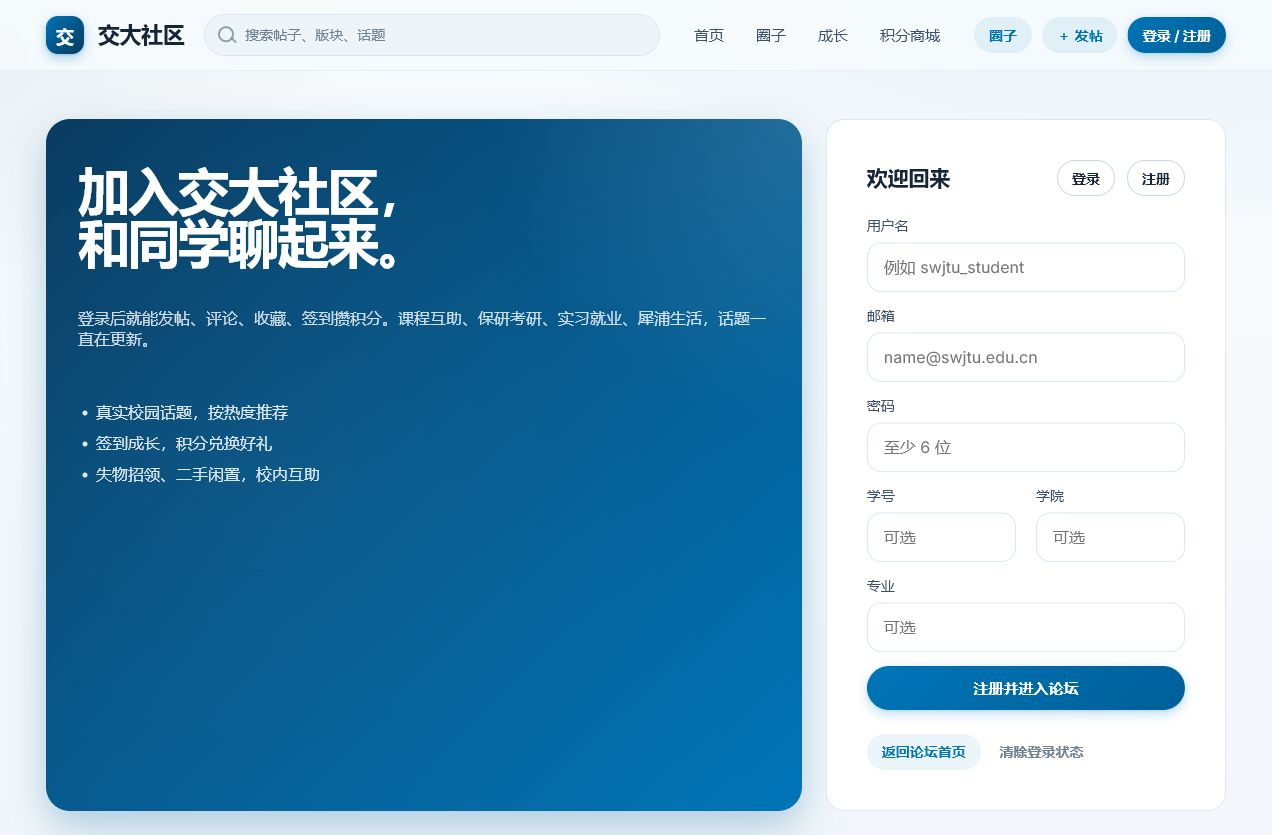
\includegraphics[width=0.88\textwidth]{figures/01_register_page.png}
\caption{用户注册页面}
\end{figure}
\begin{figure}[H]
\centering
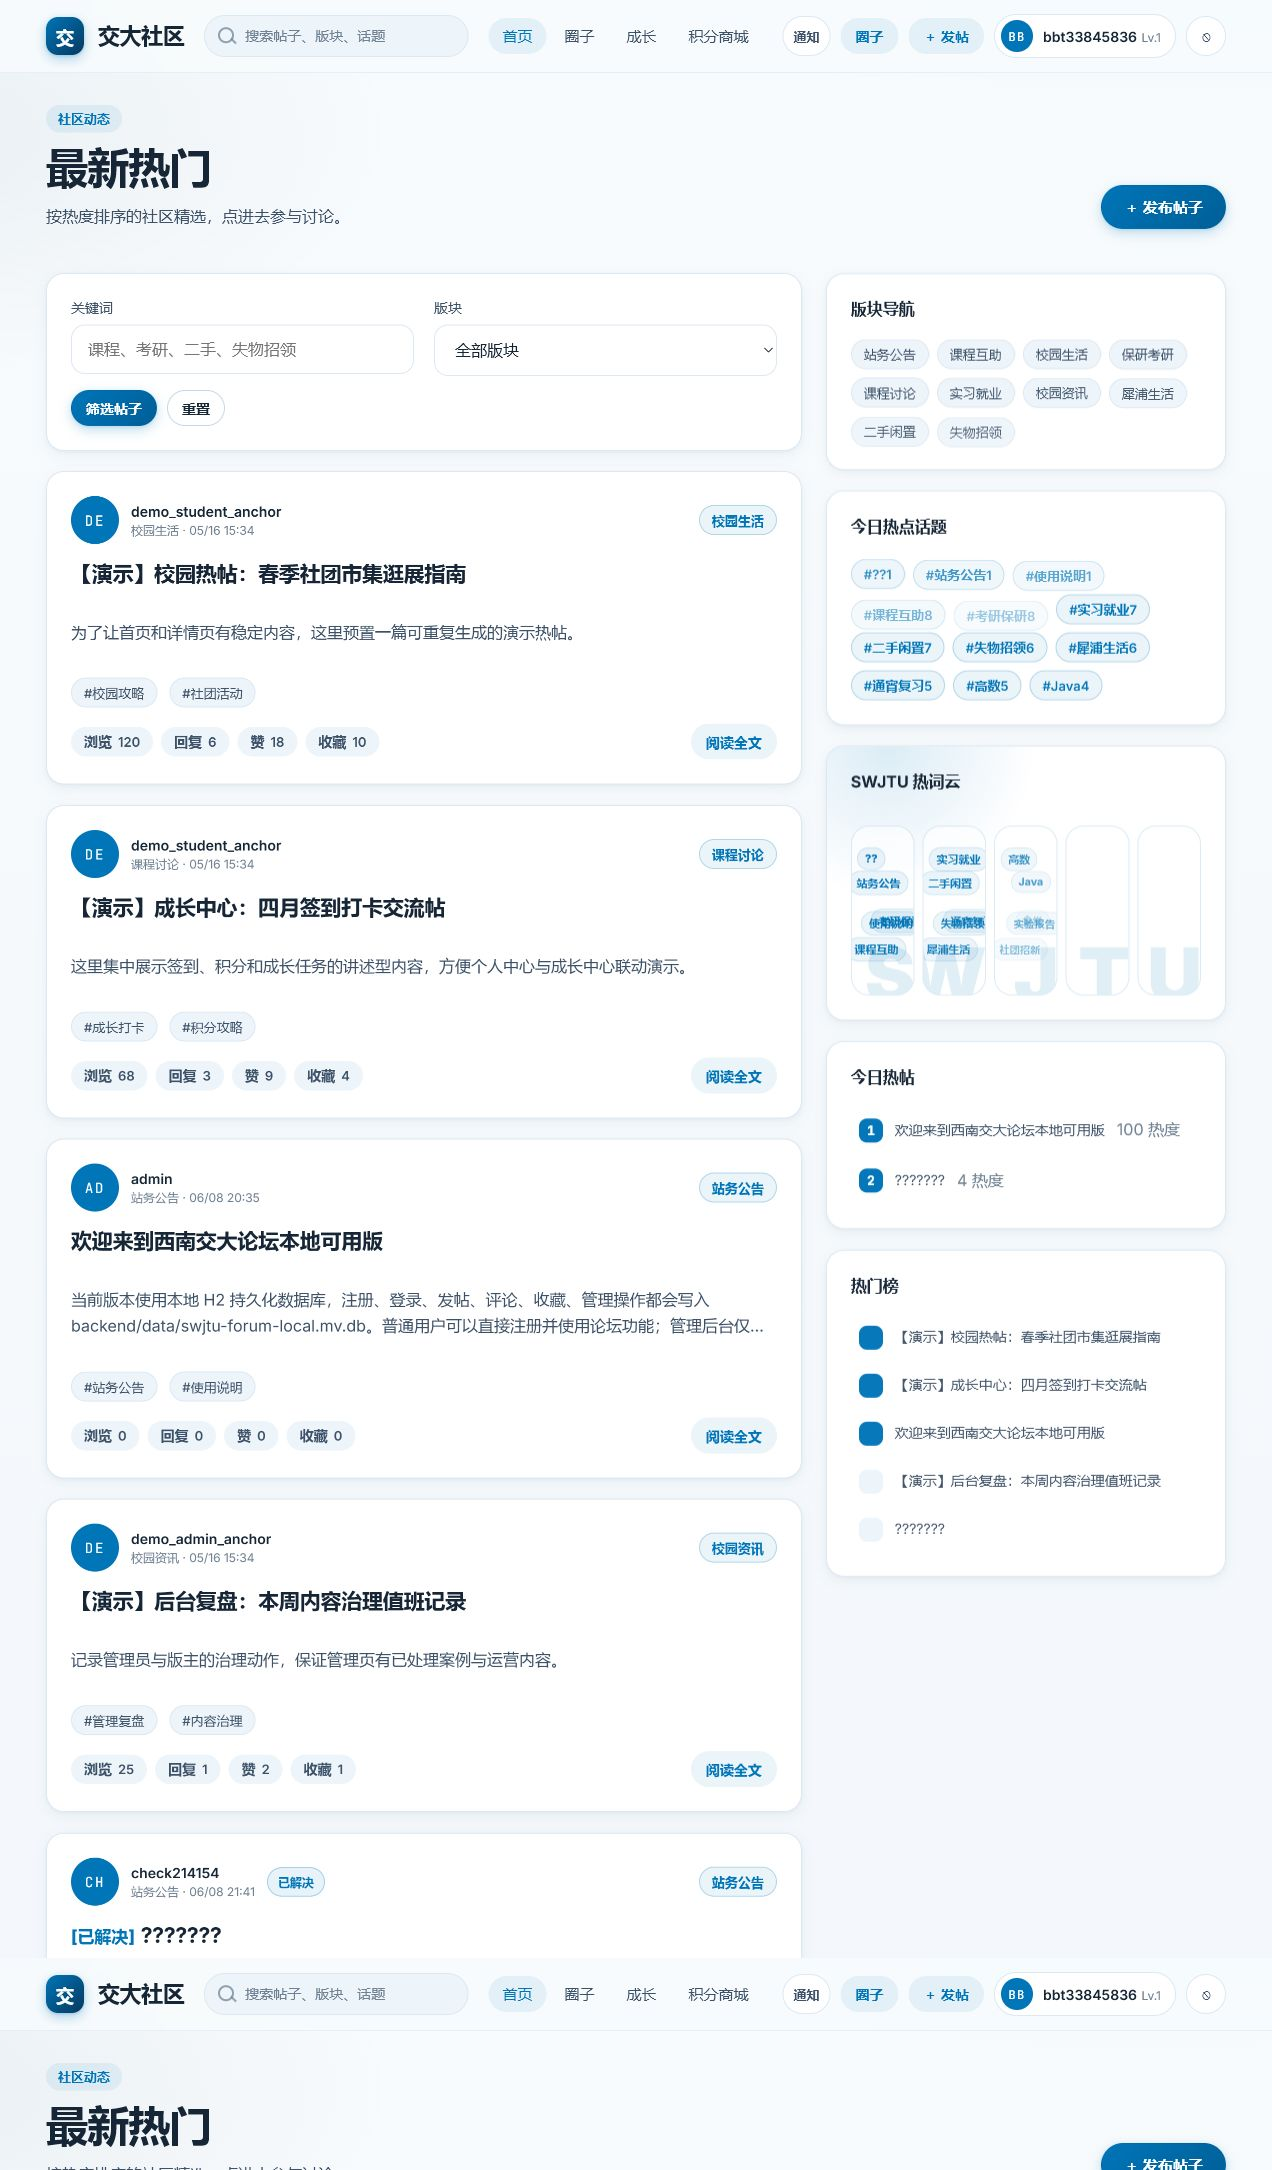
\includegraphics[width=0.88\textwidth]{figures/05_home_post_list.png}
\caption{首页帖子列表}
\end{figure}
\begin{figure}[H]
\centering
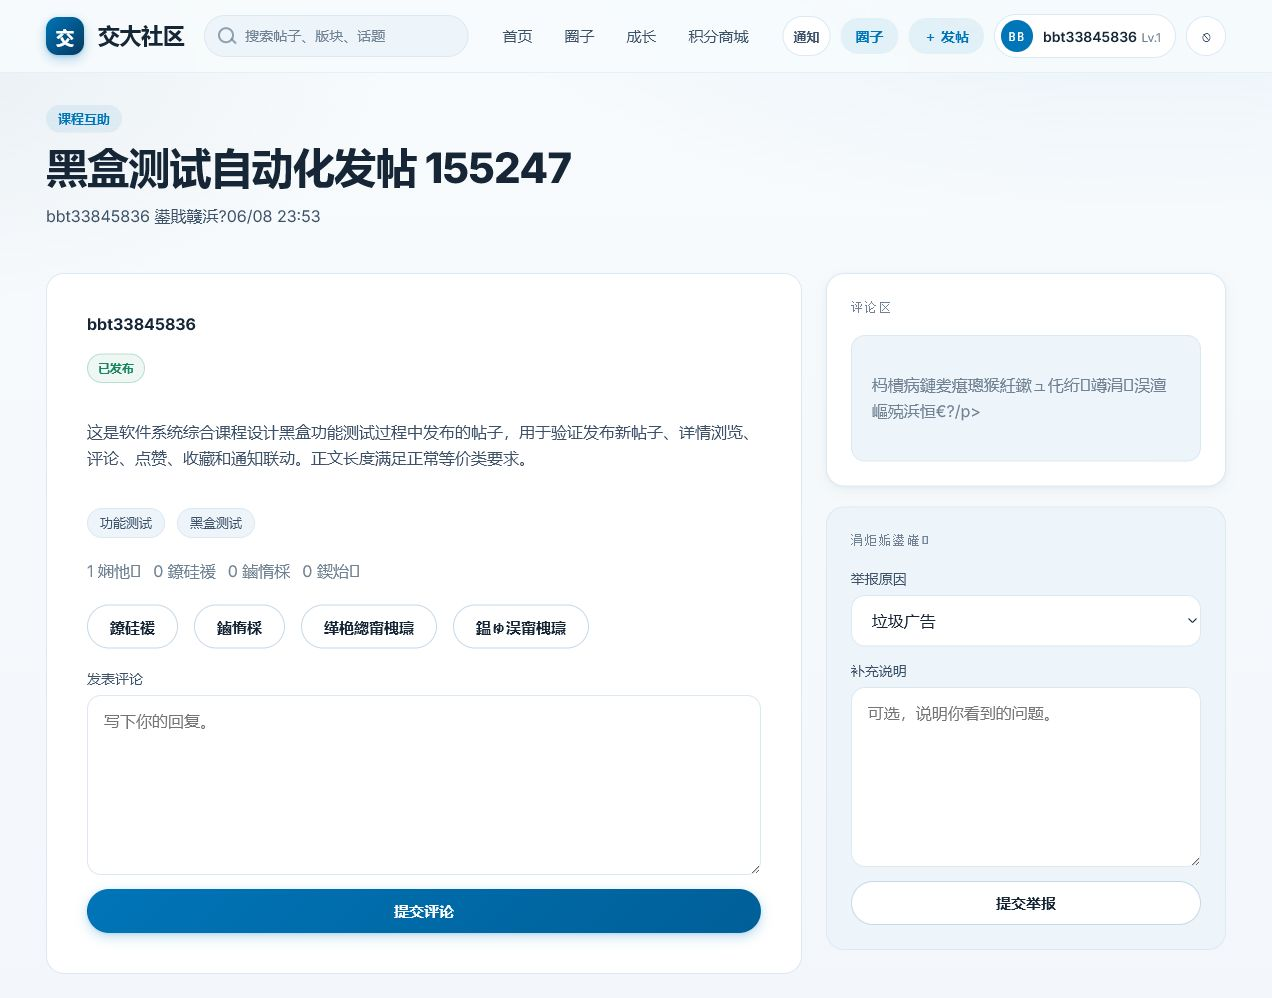
\includegraphics[width=0.88\textwidth]{figures/09_create_post_success_detail.png}
\caption{发帖成功详情页}
\end{figure}
\begin{figure}[H]
\centering
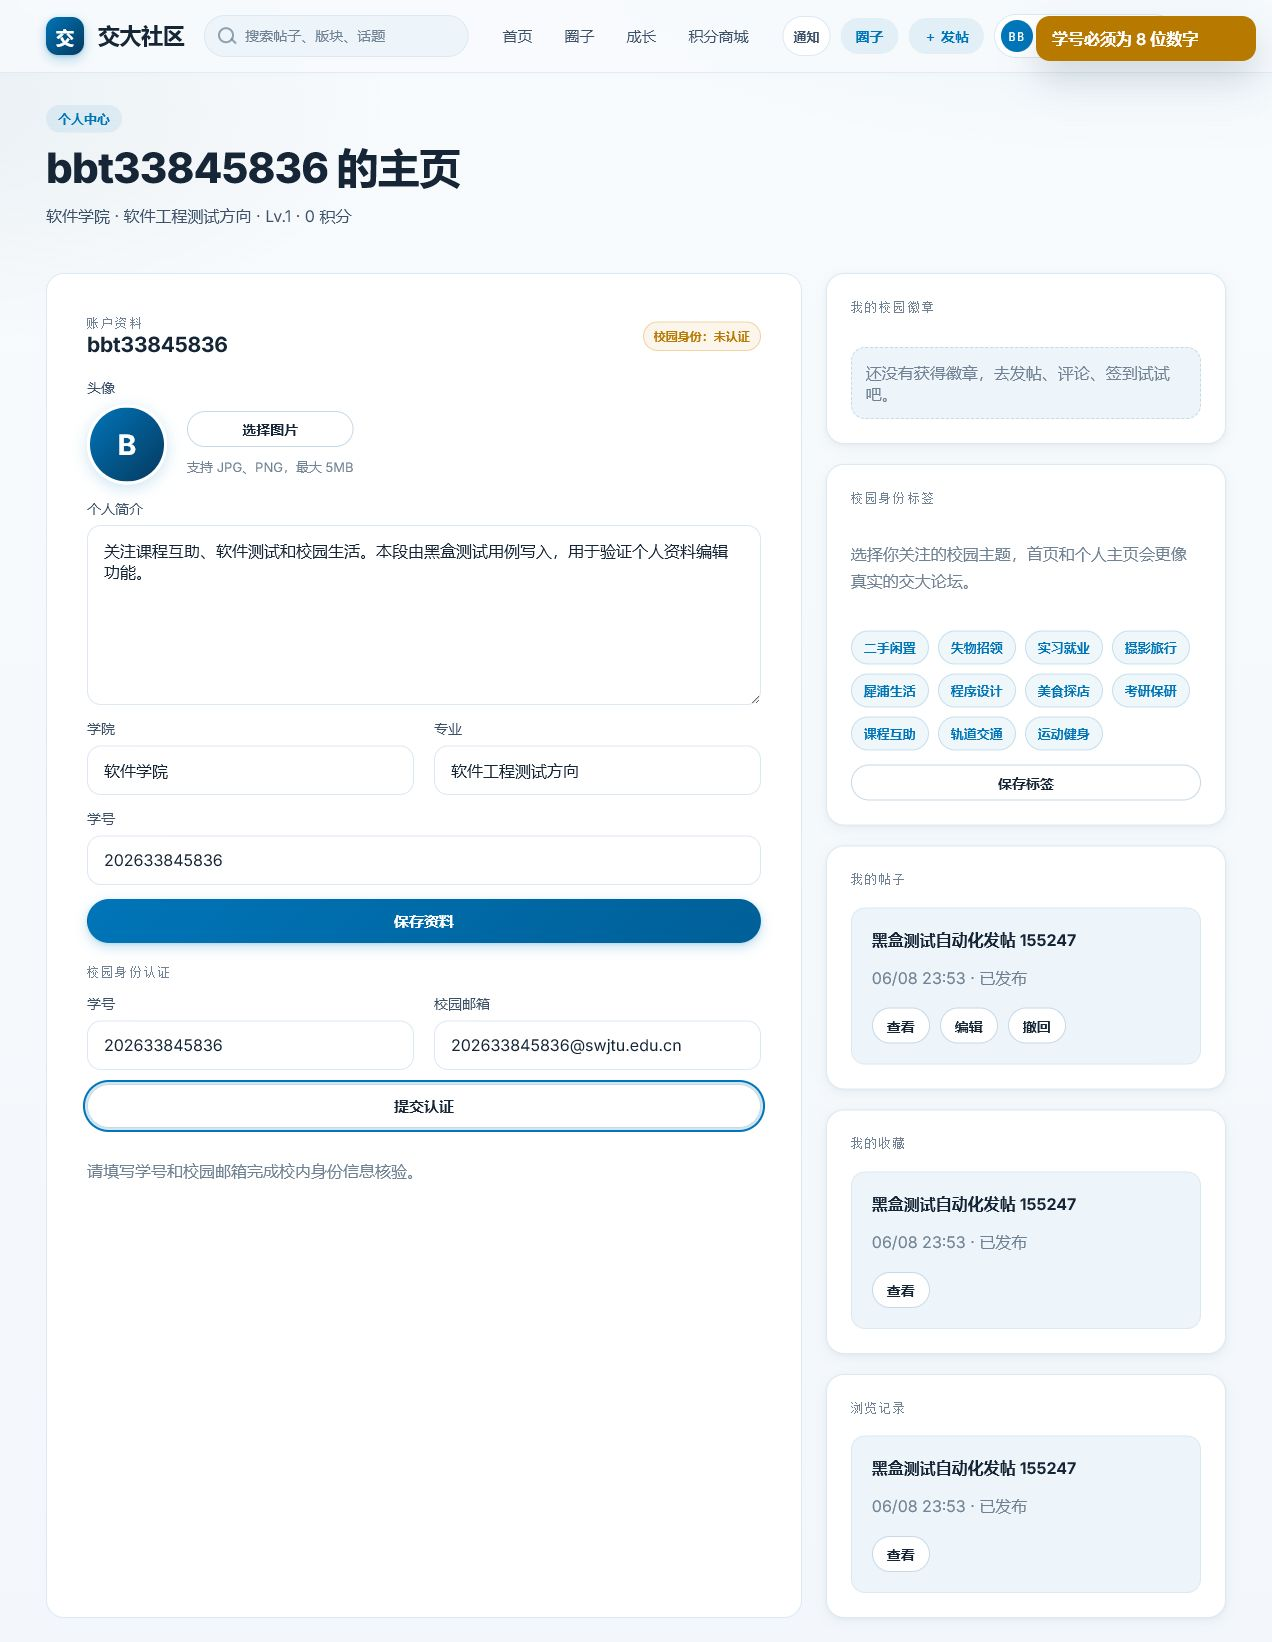
\includegraphics[width=0.88\textwidth]{figures/15_campus_identity_success.png}
\caption{校园身份认证成功}
\end{figure}
\begin{figure}[H]
\centering
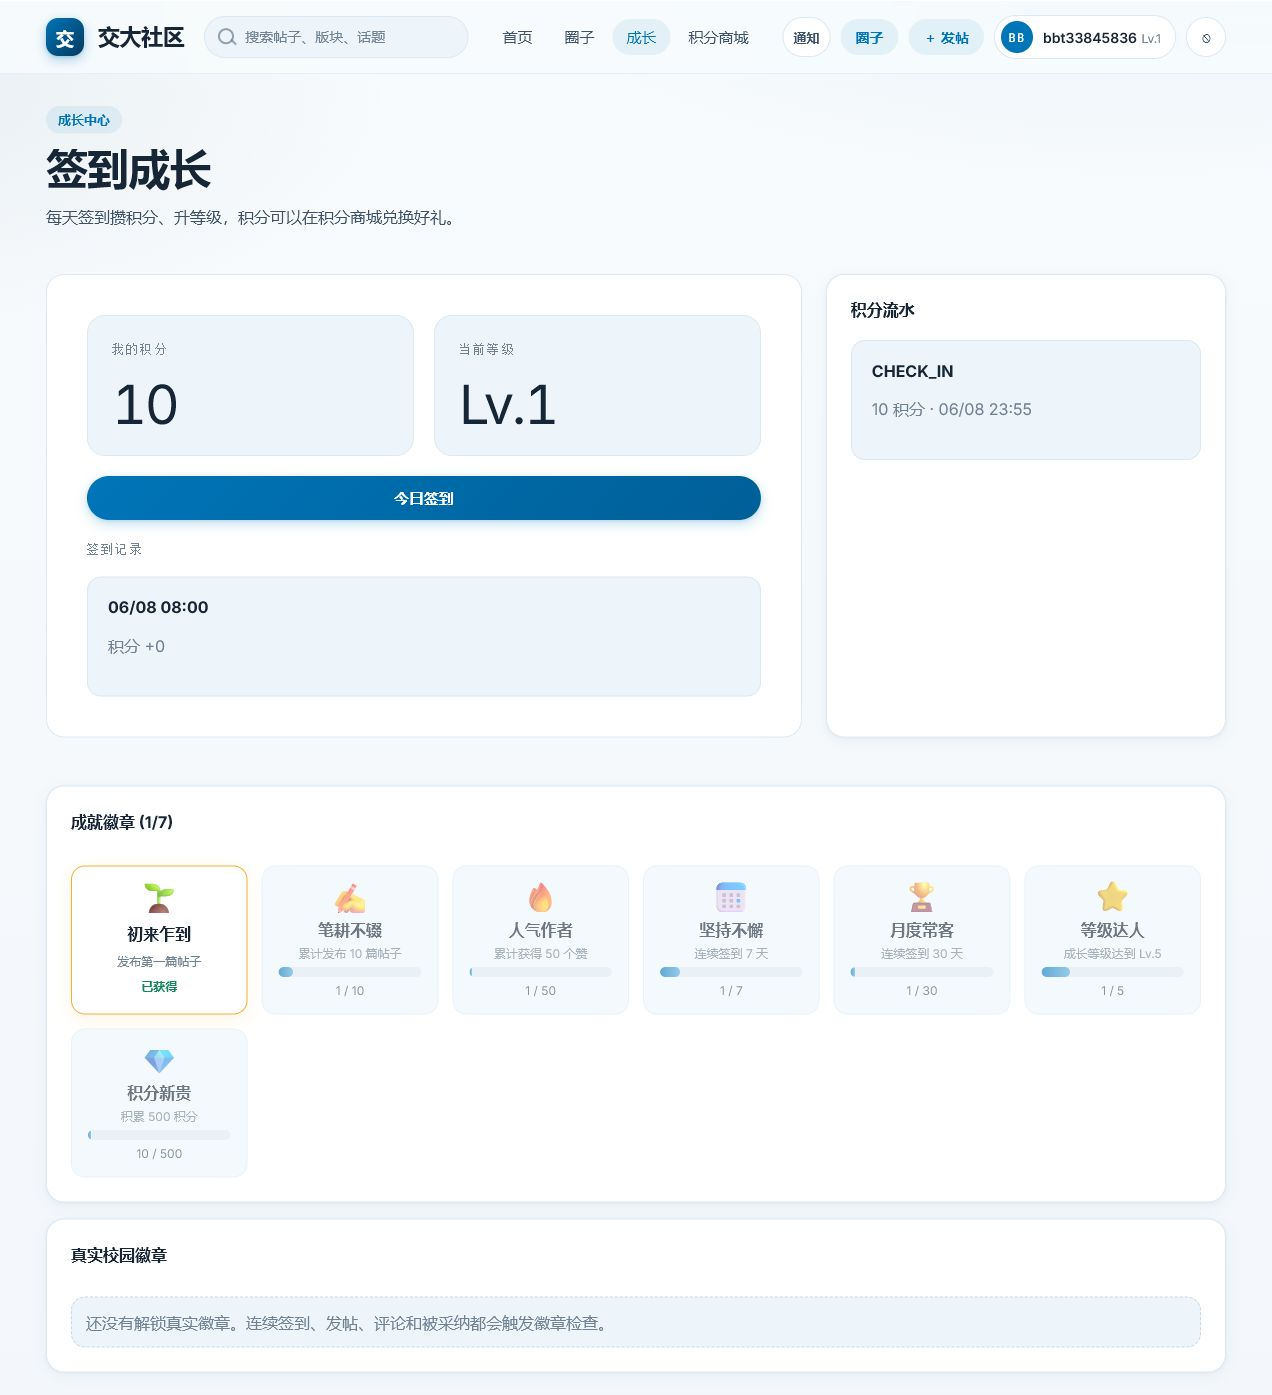
\includegraphics[width=0.88\textwidth]{figures/19_daily_checkin_success_or_repeat.png}
\caption{每日签到结果}
\end{figure}
\begin{figure}[H]
\centering
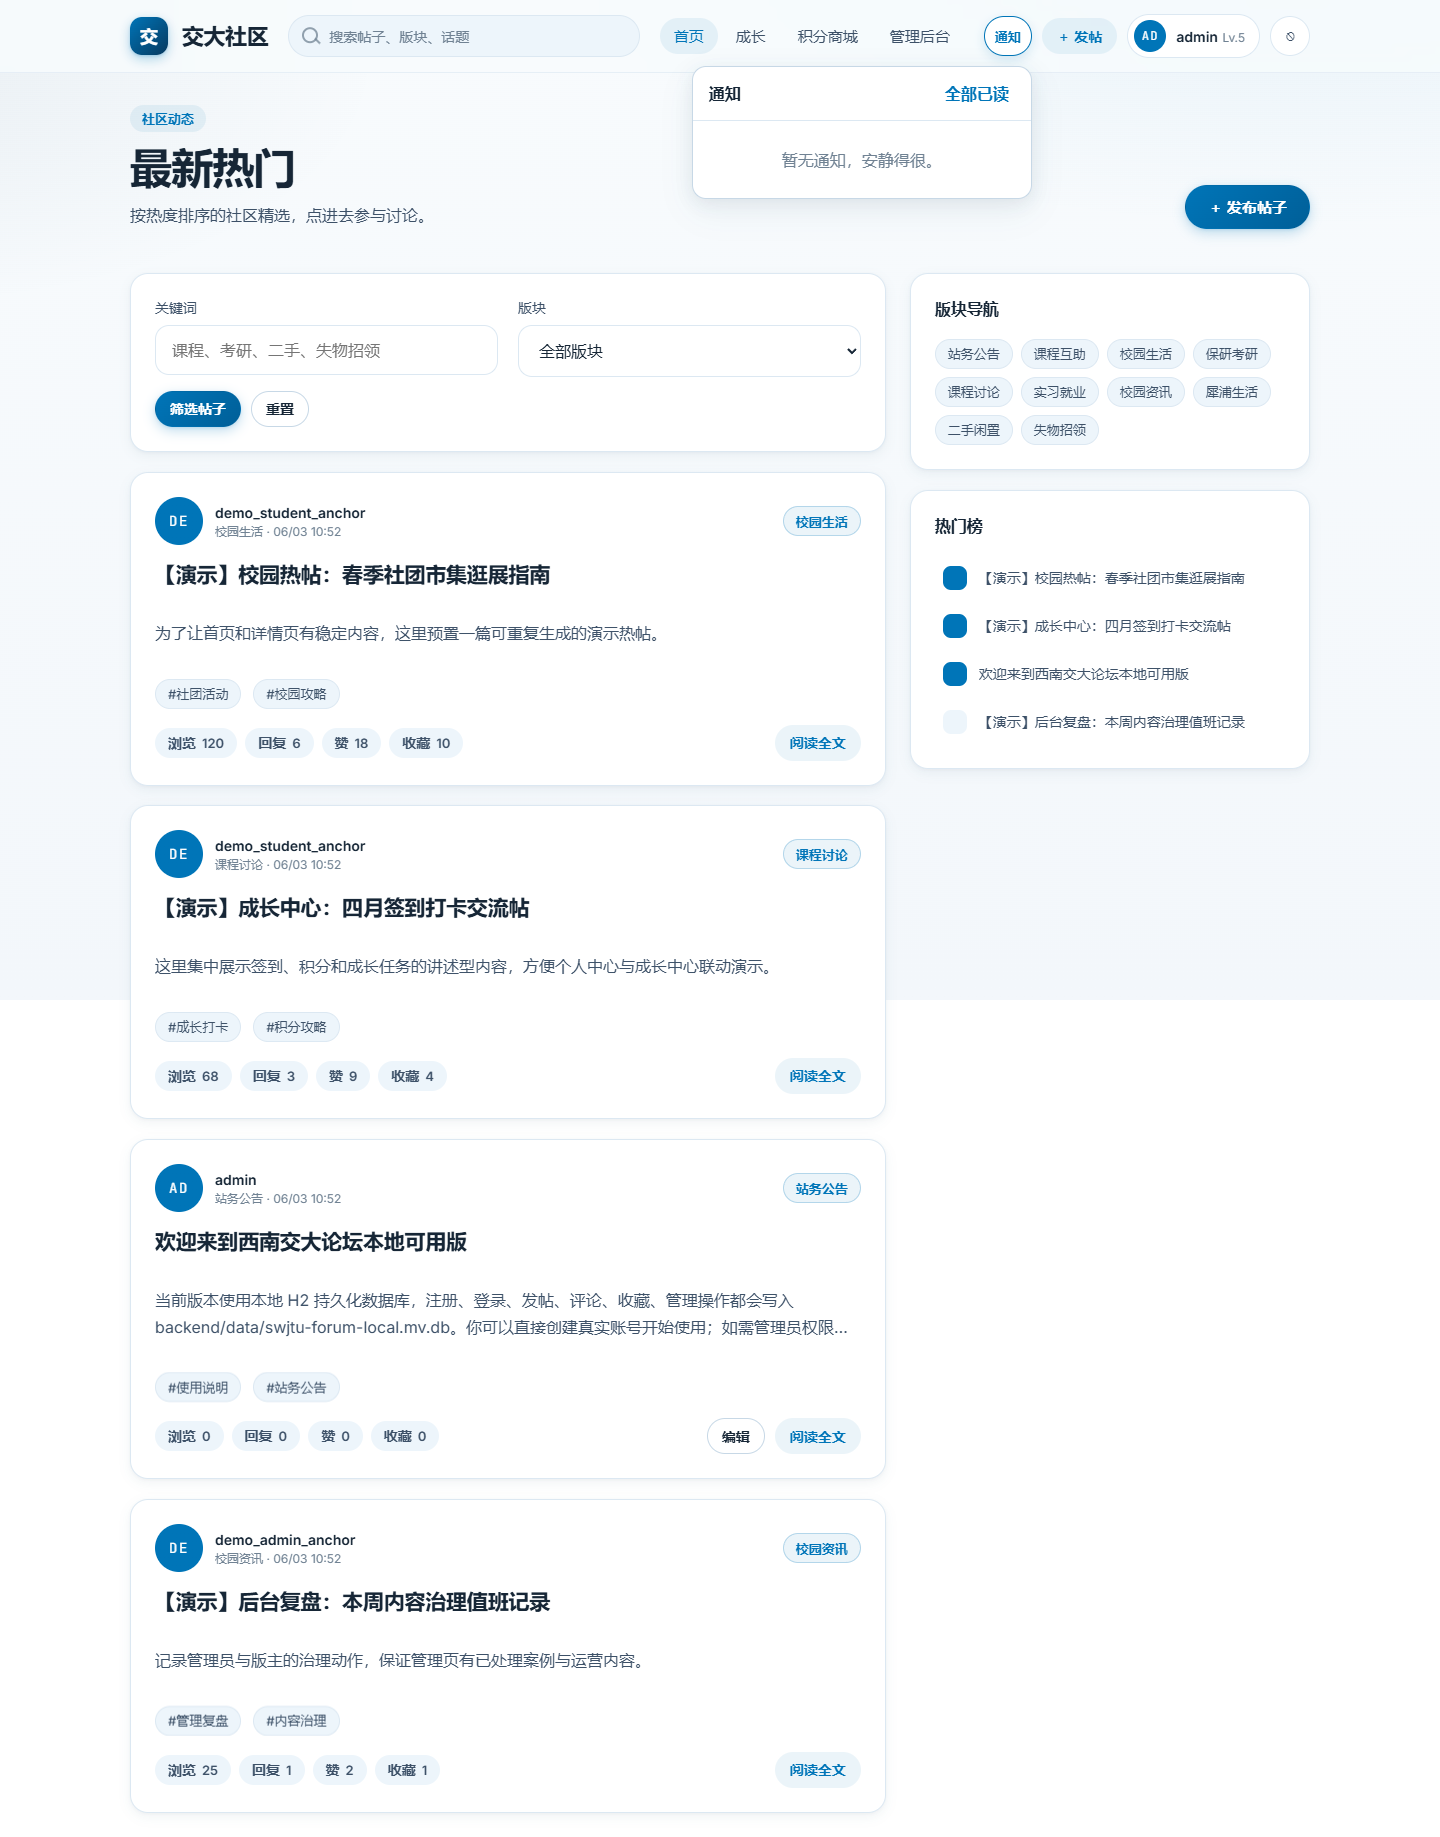
\includegraphics[width=0.88\textwidth]{figures/BUG-001-notification-desktop.png}
\caption{修复后通知中心桌面端展开}
\end{figure}
\begin{figure}[H]
\centering
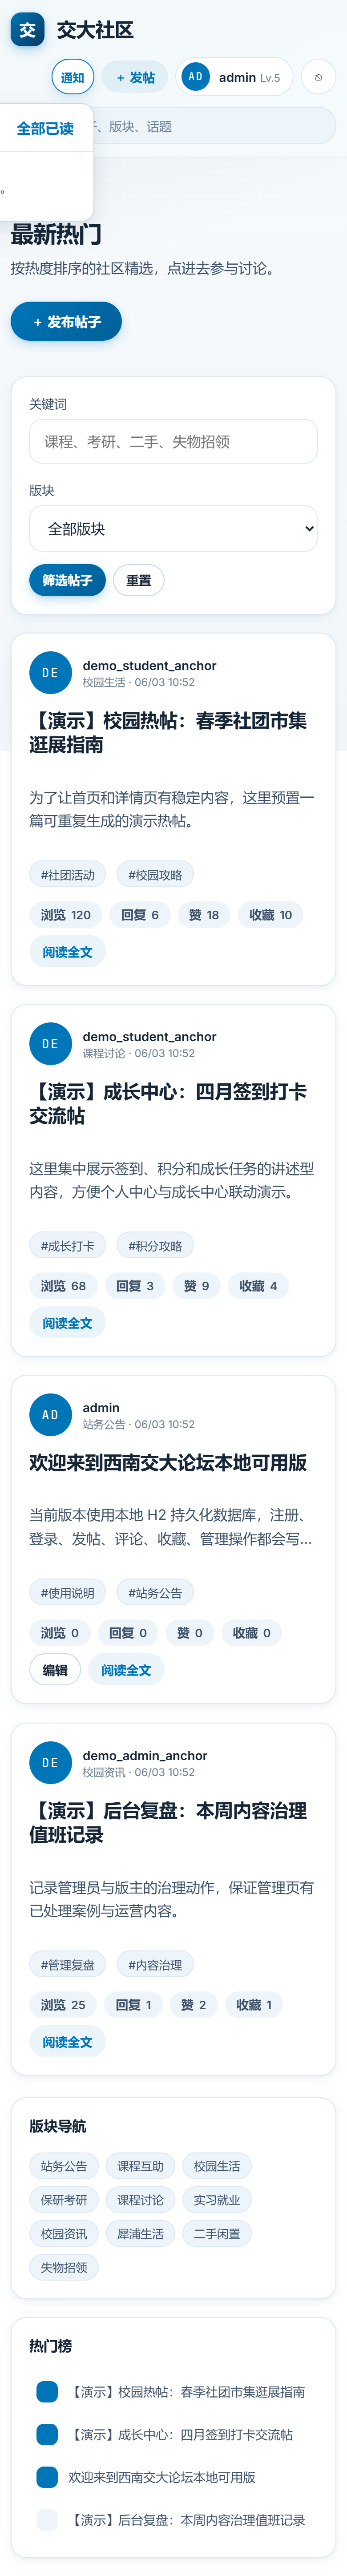
\includegraphics[width=0.88\textwidth]{figures/BUG-001-notification-mobile.png}
\caption{修复后通知中心移动端展开}
\end{figure}
\begin{figure}[H]
\centering
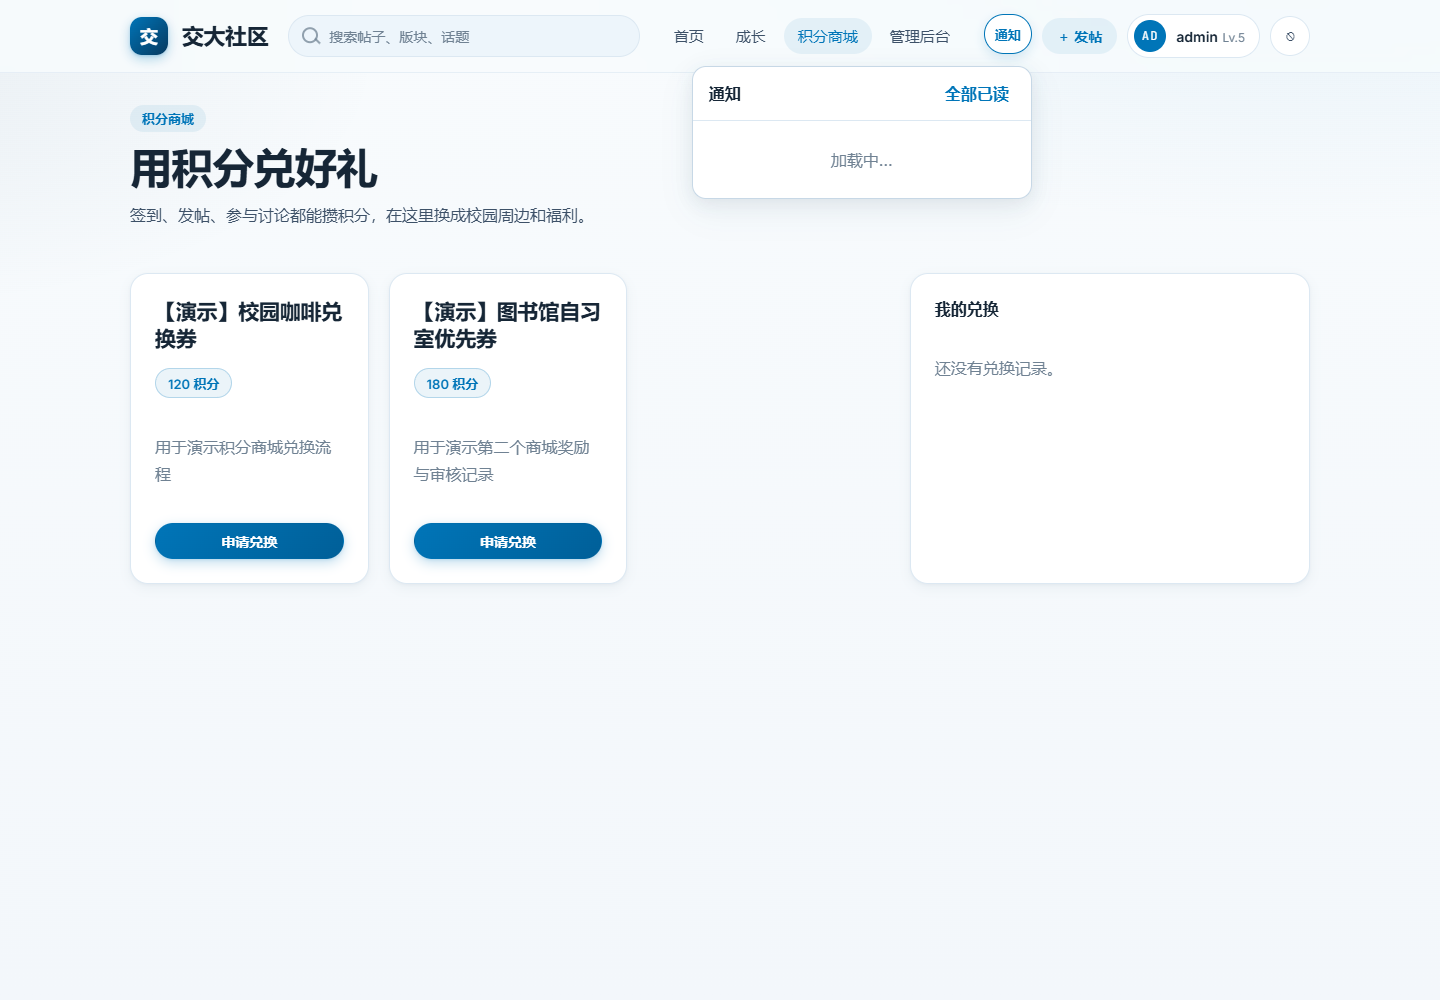
\includegraphics[width=0.88\textwidth]{figures/BUG-002-rewards-redemptions.png}
\caption{修复后积分商城和兑换记录页面}
\end{figure}

\section{缺陷清单}
\begin{longtable}{P{1.5cm}P{2.3cm}P{1.2cm}P{6.2cm}P{1.8cm}P{5.2cm}}
\toprule
编号 & 模块 & 严重 & 标题 & 状态 & 证据\\
\midrule
\endfirsthead
\toprule
编号 & 模块 & 严重 & 标题 & 状态 & 证据\\
\midrule
\endhead
BUG-001 & 通知中心 & 高 & 点击通知后面板DOM存在但仍被hidden/display:none隐藏 & 已修复 & 22\_notification\_center\_open.png;BUG-001-notification-desktop.png;BUG-001-notification-mobile.png \\
BUG-002 & 积分商城 & 高 & 兑换后刷新我的兑换记录出现500/页面加载失败 & 已修复 & 21\_rewards\_redeem\_result.png;BUG-002-rewards-redemptions.png;verification-summary.json \\
BUG-003 & 便携包启动 & 高 & 旧H2数据库升级时comments.accepted非空列无默认值导致启动失败 & 已修复 & verification-summary.json \\
BUG-004 & 发帖 & 中 & 部分详情页按钮或静态文案出现中文乱码 & 待修复 & 09\_create\_post\_success\_detail.png \\
BUG-005 & 成长系统 & 中 & 签到记录区域积分展示与积分流水不完全一致 & 待修复 & 19\_daily\_checkin\_success\_or\_repeat.png \\
BUG-006 & 个人中心 & 低 & 校园身份认证覆盖学院专业前缺少二次确认 & 待优化 & 14\_profile\_edit\_success.png;15\_campus\_identity\_success.png \\
\bottomrule
\end{longtable}

\section{修复说明与回归验证}
本轮优先修复两个会直接阻断用户使用的高严重问题。通知中心问题的根因是面板DOM虽然创建，但关闭/打开逻辑同时受内联样式和hidden属性影响，点击按钮后面板仍不可见。修复后统一使用hidden属性控制可见性，并让CSS中\texttt{.notif-panel}保持\texttt{display:flex}布局。回归截图显示桌面端和移动端均能展开通知中心。

积分商城问题的根因是兑换记录接口直接序列化JPA实体，兑换记录中的user/reward关联在部分路径下触发懒加载或循环序列化风险，导致前端刷新“我的兑换”时出现服务端错误。修复后新增\texttt{RedemptionRequestResponse} DTO，Controller返回DTO而不是实体；Repository增加关联抓取查询；Service在创建或审核兑换后返回已加载关联的记录。回归验证中\texttt{/growth/redemptions}返回200，积分商城页面刷新不再出现加载失败。

启动回归中还发现旧H2数据库升级时\texttt{comments.accepted}非空列缺少默认值会导致后端启动失败。修复方式是在实体字段上补充\texttt{boolean default false}，并重新打包便携jar。修复后后端可在既有demo数据上完成迁移并启动。

\section{脚本开发遇到的问题}
第一，便携包启动脚本在当前PowerShell环境下会受到\texttt{Path/PATH}重复环境变量影响，直接使用\texttt{Start-Process}可能失败。为保证测试稳定，实际启动采用干净环境变量的独立Java进程，并通过端口监听和HTTP 200健康检查确认服务稳定后再执行测试。

第二，前端页面包含运行时渲染逻辑，不能只等待静态HTML中的占位节点。积分商城旧占位符\texttt{data-slot=rewards-content}在运行时会被整个\texttt{main}内容替换，因此自动化脚本改为等待\texttt{app-ready}类和页面错误文本消失。

第三，截图验证必须同时检查DOM状态和视觉状态。通知中心旧问题正是DOM存在但不可见，所以本轮断言不仅检查元素存在，还检查hidden属性、计算display值和aria-expanded状态。

\section{体会与总结}
这次练习说明，黑盒测试不只是写“输入什么、输出什么”的表格。对于论坛类系统，很多严重问题发生在跨功能链路上：注册影响登录态，登录态影响发帖和互动，发帖影响通知和关注，积分影响商城兑换。单点测试只能证明按钮能点，链路测试才能发现刷新、序列化、持久化和权限控制中的缺陷。

等价类方法帮助我避免遗漏主要输入类别；边界值方法帮助我把学号长度、密码长度、积分差值、未读数等临界点单独列出；判定表方法最适合表达“登录/未登录、已关注/未关注、积分足够/不足、资源存在/不存在”这类组合条件。后续如果继续完善，应优先把150条设计用例中尚未执行的P1用例转化为自动化脚本，并补充Edge IE模式或兼容层验证。

\end{document}
